\documentclass[12pt]{article} %,fleqn
\usepackage{Diploma}
\usepackage{tikz}
\usetikzlibrary{arrows.meta,calc, chains,decorations.pathreplacing,calligraphy,positioning,quotes,shadows, shapes.geometric,snakes}
\definecolor{mydarkblue}{rgb}{0,0.08,0.55}

\definecolor{mygreen1}{rgb}{0.302,0.6863,0.2902}
\definecolor{myblue1}{rgb}{0.2157,0.4941,0.7216}
\definecolor{mybrown1}{rgb}{0.651,0.3373,0.1569}
\definecolor{myyellow1}{rgb}{1.0,1.0,0.2}
\definecolor{mypurple1}{rgb}{0.5961,0.3059,0.6392}

\tikzset{
mystyle/.style={
  circle,
  line width=1pt,
  inner sep=0pt,
  text width=2em,
  align=center,
  draw=black,
  }
}
\tikzset{
bigstyle/.style={
  circle,
  line width=1pt,
  inner sep=0pt,
  text width=3em,
  align=center,
  draw=black,
  }
}
\tikzset{
myline/.style={
  line width=1pt,
  -{Latex[length=2mm]}
  }
}
\tikzset{
bigline/.style={
  line width=1.5pt,
  -{Latex[length=2mm]}
  }
}
\tikzset{
mysnake/.style={
  decoration={snake, pre length=0.01mm, segment length=2mm, amplitude=0.3mm, post length=3mm},
  decorate
  }
}


\begin{document}

{
\renewcommand{\baselinestretch}{1}
\thispagestyle{empty}
\begin{center}
    \sc
        Министерство науки и высшего образования Российской Федерации\\
        Московский физико-технический институт\\
        {\rm(национальный исследовательский университет)}\\
        Физтех-школа прикладной математики и информатики\\
        Магистерская программа\\
        <<Методы и технологии искусственного интеллекта>>\\[35mm]
    \rm\large
        Ивченков Ярослав Павлович\\[10mm]
    \bf\Large
        Объектно-центричное представление мира агента \\
        в обучении с подкреплением\\[10mm]
    \rm\normalsize
        03.04.01 --- Прикладные математика и физика\\[10mm]
    \sc
        Магистерская диссертация\\[30mm]
\end{center}
\hfill\parbox{80mm}{
    \begin{flushleft}
    \bf
        Научный руководитель:\\
    \rm
        д. т. н\\
        Матвеев Иван Алексеевич\\[5cm]
    \end{flushleft}
}
\begin{center}
    Москва\\
    2022 г.
\end{center}
}

\clearpage
\tableofcontents

\newpage
\begin{abstract}
    В данной работе рассматриваются задача улучшения обобщающей способности алгоритмов модельного подхода в обучении с подкреплением, решающих задачу визуального роботизированного контроля. Предложены различные объектно-центричные модели мира агентов, учитывающие причинно-следственные связи между манипулятором и объектом в среде. Рассматривается семейство моделей, выделяющее в явном виде влияние манипулятора на объект и проанализированы их качества и потенциал для разных сред. Для оценки качества предложенных алгоритмов проведены эксперименты в двух наборах сред, CasualWorld и MetaWorld. Полученные результаты позволяют утверждать, что рассмотренные модели мира позволяют добиться большей обобщающей способности, чем базовый алгоритм модельного подхода.
\end{abstract}

\clearpage
%%%%%%%%%%%%%%%%%%%%%%%%%%%%%%%%%%%%%%%%%%%%%%%%%%%%%%%%%%%%%%%%%%%%%%%%%%
\section{Введение}
%%%%%%%%%%%%%%%%%%%%%%%%%%%%%%%%%%%%%%%%%%%%%%%%%%%%%%%%%%%%%%%%%%%%%%%%%%

% Введение объясняет мотивацию работы:
% где возникает данная задача,
% почему её решение так важно,
% как её решали до сих пор,
% в~чём недостатки этих решений,
% и~что нового предлагает автор.
% Введение лучше писать напоследок, так как
% в~ходе работы обычно происходит переосмысление постановки задачи.

% Вводятся на~неформальном уровне основные понятия,
% необходимые для понимания постановки задачи.
% Определяются цели исследования и~формулируется постановка задачи.

% Во~введении можно привести краткий анализ источников информации. 
% Однако если литературный обзор большой, ему лучше посвятить отдельный раздел.

% В~конце введения даётся краткое содержание работы по~разделам,
% при этом отмечается, какие подходы, методы, алгоритмы
% предлагаются автором впервые.
% Перечисляются основные результаты и~1--2 самых важных вывода работы.

% Введение может быть близко по содержанию к~тексту доклада на защите.


Обучение с подкреплением является одним из многообещающих направлений изучения искусственного интеллекта. 
Данная область науки занимается задачами последовательного принятия решений. Достаточно большое количество задач в реальной жизни подходит под это описание, например, контроль действий манипулятора, управление беспилотным автомобилем или компьютерные игры. 
В каждой из подобных задач можно выделить две основные сущности, взаимодействующие друг с другом - агента и среду. 
Агент может получать от среды информацию различного типа на каждом шаге - например, вектор позиций конечностей манипулятора или картинку с камеры автомобиля. 
Как и в остальных областях машинного обучения, работа с визуальными данными требует особых решений. 
В последние годы были достигнуты значительные успехи в решении подобного рода задач - в частности, в 2015 году были достигнуты  результаты, сравнимые с человеческими в играх Atari, а позже -  побиты результаты игры в Starcraft 2 и Dota 2. 
Несмотря на подобные успехи, применение алгоритмов обучения с подкреплением в реальной жизни достаточно ограничено по причине имеющихся недостатков большинства подходов. 
Для алгоритмов RL свойственно требовать очень большое количество взаимодействия со средой, они обладают плохой обобщающей способностью а также плохо интерпретируются. 
Обобщающая способность является чрезвычайно важным свойством моделей, от которого напрямую зависит возможность применения алгоритма для реальных задач, а не только в искусственных средах.

Одним из способов преодолеть данные недостатки является построение модели среды, с которой взаимодействует агент. 
Улучшение качества модели среды позволяет алгоритму проще адаптироваться к новым задачам в той же среде. 
Однако без специальных модификаций, направленных на улучшение обобщающих способностей, данные алгоритмы все равно показывают слабые обобщающие способности.

За последние годы было предложено много методов улучшения обобщающих способностей алгоритмов в этой области, доминирующим направлением в них является предобучение алгоритма с целью максимизации определенного внутреннего информационного показателя качества. 
Максимизируя их, алгоритм более эффективно исследует среду и выучивает более богатую и устойчивую модель среды, что позволяет ему избежать переобучения для определенной функции награды. 
Данный подход - предтренировка алгоритма - был успешно адаптирован из другой области машинного обучения, машинного зрения.

Во многих задачах, рассматриваемых в машинном зрении, таких как генерация сцен и генерация видео, в последние годы успешно применяется объектно-центричный подход, заключающийся в выделении на изображении отдельных сущностей. 
Введение подобного рода структуры позволяет упростить моделирование отдельных компонент изображения и сделать этот процесс более интерпретабельным. 
Также данный подход выглядит весьма уместным и перспективным в случаях, когда объекты зависят друг от друга, позволяя моделировать причинно-следственные связи.

В обучении с подкреплением объектно-центричный подход известен достаточно давно, однако исследований в данном направлении велось достаточно мало. Несмотря на то, что не во всех задачах можно с успехом выделить отдельные объектные сущности, в задачах роботизированного контроля переход к подобного рода абстракциям достаточно тривиален. 
В среде подразумевается присутствие манипулятора и, опционально, некоторого количества объектов, с которыми манипулятор может взаимодействовать.

Модели мира могут получать большие преимущества от переиспользования смоделированной или заранее заданной структуры среды \cite{WM}.
В связи с этим представляется достаточно перспективным внедрение объектно-центричного подхода в алгоритмах, основанных на модели среды, решающих задачи роботизированного контроля, в которых агент получает в качестве наблюдений изображения среды.
Тогда как его влияние на скорость обучения в решении конкретных задач не очевидно, обобщающие способности алгоритмов должны возрасти за счет отдельного моделирования динамик объектов на изображении.
% - задача, в которой, управляя манипулятором и получая в качестве наблюдений изображения среды, агенту необходимо достичь заранее поставленную цель, например переместить кубик в определенное место. 

\clearpage
%%%%%%%%%%%%%%%%%%%%%%%%%%%%%%%%%%%%%%%%%%%%%%%%%%%%%%%%%%%%%%%%%%%%%%%%%%
\section{Обзорно-постановочный раздел работы}
%%%%%%%%%%%%%%%%%%%%%%%%%%%%%%%%%%%%%%%%%%%%%%%%%%%%%%%%%%%%%%%%%%%%%%%%%%

% Заголовки разделов и подразделов в~данном документе приводятся для примера
% и~должны быть заменены на более содержательные, отражающие суть работы.
% Можно оставить <<Введение>> и <<Заключение>>.

% \subsection{Основные понятия и определения}
% Вводятся общепринятые понятия и~обозначения со~ссылками на~литературу.

% \subsection{Обзор современного состояния проблемы}
% Излагаются известные результаты со~ссылками на~литературу.
% Необходимые для дальнейшего известные факты
% могут формулироваться как теоремы без доказательств, но~со~ссылками на~источники.

% \begin{Def}
%     Математический текст \emph{хорошо структурирован},
%     если в~нём выделены определения, теоремы, утверждения, примеры, и~т.\,д.,
%     а~неформальные рассуждения (мотивации, интерпретации)
%     выделены в~отдельные подпараграфы
%     (для этого хорошо подходит команда \verb|\paragraph{|\emph{текст}\verb|}|).
% \end{Def}

% \begin{Corollary}
%     Надо уделять большое внимание не~только формальному изложению,
%     но~и~неформальным мотивациям и~интерпретациям результатов.
%     Иначе основные идеи работы невозможно будет понять быстро.
% \end{Corollary}

% \begin{Corollary}
%     Основные идеи Вашего текста должны оставаться в~целом понятными, если читать его, пропуская все формулы.
% \end{Corollary}

% \begin{Remark}
%     Здесь показано применение окружений
%     Def, Theorem, Corollary, Remark.
% \end{Remark}

% \subsection{Формальная постановка задачи}
% К данному моменту читатель ознакомлен со всеми необходимыми понятиями
% и~подготовлен к~точным формулировкам задач, решаемых автором в~данной работе.

\subsection{Основные понятия и определения}
Обучение с подкреплением занимается задачами последовательного принятия решений. 
Данная задача в большинстве случаев формализуется в терминах Марковского Процесса Принятия Решений (МППР), определяющегося следующим образом:
\begin{Def}
    Марковский Процесс Принятия Решений (МППР) задается кортежем из четырех элементов $\mathcal{M} = \left<\mathcal{S}, \mathcal{A}, P, \mathcal{R}\right>$, где:
    \begin{itemize}
        \item $\mathcal{S}$ - набор состояний;
        \item $\mathcal{A}$ - набор действий;
        \item $P(s_{t+1}\mid s_t, a_t)$ - функция перехода состояний среды;
        \item $\mathcal{R}(s_t, a_t, s_{t+1})$ - функция вознаграждения среды;
    \end{itemize}
    \label{mdp}
\end{Def}
В работе рассматривается случай конечного МППР с вероятностной функцией перехода состояний. 
Состояние и действие предполагаются конечномерными векторами $s_t \in \mathbb{R}^{d_{s}}, a_t \in \mathbb{R}^{d_{a}}$.

Поведение агента определяется действиями, совершаемыми им в тех или иных состояниях среды. 
Агент принимает их в соответствии со \textit{стратегией} $\pi (a \mid s)$, представляющей собой функцию, ставящую в соответствие каждому состоянию среды $s_t$ действие, которое агент должен предпринять. 
В общем виде эта функция имеет вид вероятностного распределения над множеством действий.

Для полного определения задачи обучения с подкреплением также необходимо задать оптимизируемый функционал.
Вводится понятие \textit{коэффициента дисконтирования} $\gamma \in \left[0,1\right]$, отвечающего за уменьшение текущей ценности награды, которую агент может получить в будущем. Используя это понятие, формулируется следующее:
 \begin{Def}
    Отдача $R(\tau) = \sum_{t=0}^{T}\gamma^t r_t$ - дисконтированная сумма вознаграждений на определенной траектории $\tau$.
 \end{Def}
Отдача является случайной величиной, поскольку и выбор действий агентом, и функция перехода состояний среды могут иметь случайный характер в общем случае. 
Таким образом, от стратегии агента ожидается, что матожидание отдачи по всем траекториям, которые мы можем получить, будет максимальным. 
Формально это выражается следующим образом:
\begin{Def}
    Целевая функция, определяемая как $G(\pi, \mathcal{M}) = \mathbb{E}_{\tau \sim \pi}\left[R\left(\tau\right)\right] = \mathbb{E}_{\pi}\sum_{t}\gamma^t r_t$, есть математическое ожидание отдачи за эпизод, полученный при помощи использования агентом стратегии $\pi$. 
\end{Def}
Задача агента в обучении с подкреплением в общем случае - максимизировать целевую функцию $G(\pi, \mathcal{M})$ путем изменения стратегии $\pi$.
Для упрощения задачи вводится \textit{функция полезности} $V^{\pi}(s) = \mathbb{E}_{s_o=s,\tau \sim \pi}\left[R(\tau)\right] = \mathbb{E}_{s_o=s,\tau \sim \pi}\left[\sum_{t=0}^{T}\gamma^t r_t\right]$, означающая ожидаемую отдачу в эпизоде, если агент следует стратегии $\pi$ и стартует из состояния $s$. Алгоритмы, фокусирующиеся на модели среды, также пытаются аппроксимировать истинную функцию перехода состояний $P(s_{t+1} \mid s_t, a_t)$ своей собственной \textit{моделью среды} $\mathit{P}(s' \mid s, a)$. Также возможно моделирование функции награды $\mathit{R}(s', a, s)$ различного вида.
Совокупность моделей, использующихся алгоритмом, называется \textit{моделью мира}.

В постановке задачи, использующей МППР, подразумевается, что получаемые агентом состояния $s_t^{agent}$ и состояния среды $s_t^{env}$ одинаковы, то есть агент имеет доступ к истинному состоянию среды.
Однако в большинстве ситуаций, в особенности практических, получить такое состояние затруднительно либо вообще невозможно, например, когда агент получает в качестве наблюдения изображение с камеры.
Данный факт вынуждает разделить понятия наблюдений, получаемых агентом, и состояний среды, что приводит к новой обобщенной формулировке: 
\begin{Def}
    Частично Наблюдаемый Марковский Процесс Принятия Решений задается кортежем из шести элементов $\mathcal{M} = \left<\mathcal{S}, \mathcal{A}, P, \mathcal{R}, \Omega, \mathcal{O} \right>$, где:
    \begin{itemize}
        \item $\mathcal{S}$ - набор состояний;
        \item $\mathcal{A}$ - набор действий;
        \item $P(s_{t+1} \mid s_t, a_t)$ - функция перехода состояний среды;
        \item $\mathcal{R}(s_t, a_t, s_{t+1})$ - функция вознаграждения среды;
        \item $\Omega(o_t \mid s_t)$ - функция наблюдений;
        \item $\mathcal{O}$ - множество наблюдений.
    \end{itemize}
    \label{pomdp}
\end{Def}

Предполагается, что состояние $s_t$ является функцией от истории эпизода $H_t = a_0, o_1, a_1, \dots, a_{t-1}, o_t$, такой, что $s_t = f(H_t)$ сохраняет всю информацию эпизода, необходимую для максимально возможно точного предсказания $o_{t+1}$. 
Определенное таким образом состояние $s_t$ сохраняет Марковское свойство, следовательно, может использоваться для получения всех результатов для стандартного МППР. 
Поскольку функция $f$ должна быть как можно менее дорогой в вычислительном плане, её ищут в виде:
\begin{equation}
\label{eq:pomdp-model}
    s_{t+1} = p(s_t, a_t, o_{t+1})
\end{equation}
Алгоритмы модельного подхода, в основе которых лежит частично наблюдаемый МППР, аппроксимируют как функцию перехода внутренних состояний среды вида 
$\mathit{P}(s' \mid s, a)$, так и функцию вида \ref{eq:pomdp-model}.

Для измерения обобщающей способности алгоритмов удобно использовать понятие контекстного МППР \cite{CMDP}:
\begin{Def}
    Контекстный МППР задается кортежем из четырех элементов $\left<\mathcal{С}, \mathcal{S}, \mathcal{A}, \mathcal{M}\left(c\right)\right>$, где:
    \begin{itemize}
        \item $\mathcal{C}$ - множество контекстов;
        \item $\mathcal{S}$ - множество состояний;
        \item $\mathcal{A}$ - множество действий;
        \item $\mathcal{M}$ - отображение из множества контекстов $c \in \mathcal{C}$ в МППР $\mathcal{M}(c)=\left(\mathcal{S}, \mathcal{A}, p^{c}(y \mid x, a), r^{c}(x), \pi_{0}^{c}\right)$
    \end{itemize}
    \label{cmdp}
\end{Def}
Контекст является скрытой переменной, определяющей конкретную задачу в контекстном МППР. 
Каждое значение контекста определяет состояния, которые могут быть встречены в эпизоде.
Отдельные части среды могут быть параметризованы значением произвольного вектора, например, значение массы какого-либо объекта. 
В этом случае, масса может быть включена в значение контекста, либо может считаться частью стохастичности среды.

Объектно-центричный подход в обучении с подкреплением не имеет устоявшейся теоретической базы. Общей чертой является разделение состояния $s_t$ на кортеж из нескольких состояний $(s_t^1, s_t^2, \dots, s_t^n)$, каждое из которых соответствует состоянию отдельной объектной сущности. В данной работе рассмотрен именно этот случай, без дополнительного разделения пространства действий. 

Возможность комбинирования объектно-ориентированного и модельного подходов заключается в возможности факторизации функций перехода состояний. В общем случае для этого используются графовые сети, однако для более простых случаев, например, взаимодействия манипулятора и единственного объекта, можно искусственно ввести причинно-следственные связи в модель мира. Благодаря этому ожидается прирост обобщающей способности алгоритма и увеличение интерпретабельности.

\subsection{Обзор современного состояния проблемы}
Поскольку работа представляет собой применение идей объектно-центричного подхода к алгоритмам обучения с подкреплением модельного подхода, будут описаны современные подходы в обоих областях.
Особое внимание уделено описанию моделей мира в работах объектно-центричного подхода.

\subsubsection{Модельный подход в обучении с подкреплением}
Серия работ \cite{planet, dreamer, dreamerv2} является одной из наиболее заметных за последние годы в модельном подходе. 
Первой в серии статей является \cite{planet}, в которой предложена новая модель мира RSSM (Recurrent State-Space Model).
Марковские состояния моделируются при помощи апостериорного распределения следующего вида:
\begin{equation}
    q\left(s_{1:T} \mid o_{1:T}, a_{1:T}\right) = 
    \prod_{t=1}^{T} q\left(s_t \mid s_{t-1}, a_{t-1}, o_t\right)
\end{equation}
По имеющимся действиям $a_{1:T}$ и наблюдениям $o_{1:T}$ вариационный автокодировщик $q$ выводит скрытые состояния $s_{1:T}$.
Имплементация $q\left(s_t \mid s_{t-1}, a_{t-1}, o_t\right)$ выдает параметры для гауссовского распределения, случайной реализацией которого является следующее состояние $s_t$.
Используя полученный автокодировщик, авторы выводят нижнюю вариационную границу для правдоподобия наблюдений:
\begin{align}
\quad &\ln p\left(o_{1: T}, r_{1: T} \mid a_{1: T}\right) 
\notag
\\
\triangleq &\ln \int \prod_{t} p\left(s_{t} \mid s_{t-1}, a_{t-1}\right) p\left(o_{t} \mid s_{t}\right) p\left(r_{t} \mid s_{t}\right) \mathrm{d} s_{1: T} 
\notag
\\
\geq &\sum_{t=1}^{T} \Big(\mathrm{E}_{q\left(s_{t} \mid o_{\leq t}, a_{<t}\right)}\left[\ln p\left(o_{t} \mid s_{t}\right) + \ln p\left(r_{t} \mid s_{t}\right)\right] \hookleftarrow
\notag
\\
- &\mathbb{E}\left[\operatorname{KL}\left[q\left(s_{t} \mid o_{\leq t}, a_{<t}\right) \| p\left(s_{t} \mid s_{t-1}, a_{t-1}\right)\right]\right]\Big) .
\label{eq:elbo}
\end{align}

Наибольший интерес представляет анализ различных архитектур состояний и функций, при помощи которых организовано взаимодействие между ними.
Авторы находят, что реализация функции переходов состояний только при помощи вероятностных распределений не является оптимальным решением.
Из-за вероятностного характера функции переходов, запоминание информации, произошедшей некоторое количество шагов назад, не является простой задачей.
Теоретически, модель может имитировать поведение детерминированной функции, однако выучить параметры таких распределений может быть проблематичным.
С другой стороны, детерминированная функция переходов, хотя и решает проблемы вероятностной, не учитывает возможной стохастики среды.

Учитывая все вышеперечисленное, авторы приходят к выводу об уместности разделения состояния на две части, одна из которых, $h_t$, генерируется при помощи детерминированной функции, а другая, $z_t$, является параметризованным распределением:
\begin{align}
& \text { Детерминированная модель переходов: } & h_{t}=f_{\phi}\left(h_{t-1}, z_{t-1}, a_{t-1}\right) 
\notag
\\
& \text { Вывод стохастической части: } & z_{t} \sim q_{\phi}\left(z_{t} \mid h_{t}, o_{t}\right) 
\notag
\\
& \text { Генерация стохастической части: } & \hat{z}_{t} \sim p_{\phi}\left(\hat{z}_{t} \mid h_{t}\right) 
\notag
\\
& \text { Декодер изображения: } & \hat{o}_{t} \sim p_{\phi}\left(\hat{o}_{t} \mid h_{t}, z_{t}\right) 
\notag
\\
& \text { Декодер награды: } & \hat{r}_{t} \sim p_{\phi}\left(\hat{r}_{t} \mid h_{t}, z_{t}\right)
\end{align}
где функция $f_{\phi}\left(h_{t-1}, z_{t-1}, a_{t-1}\right)$ является рекуррентной нейронной сетью.
Можно рассматривать $h_t$ и $z_t$ как части состояния среды, ответственные за динамику и наблюдения соответственно, поскольку во многих задачах динамика имеет более детерминированный характер, а наблюдения обладают явно выраженной стохастикой.
Авторы подчеркивают, что при выводе состояния $z_t$ необходимо получить это состояние как реализацию случайной величины из полученного распределения, чтобы не допустить детерминированного прохода информации от наблюдения $o_t$ к реконструкции $\hat{o}_t$.
Эксперименты демонстрируют, что и стохастическая часть состояния $z_t$, и детерминированная часть $h_t$ важны для успешного решения задач, в частности, без $z_t$ процесс обучения модели не приносит результатов.

В следующей статье \cite{dreamer} авторы предлагают один из сильнейших современных модельных алгоритмов, Dreamer, в основе которого лежит предложенная в прошлой статье модель мира RSSM.
Главное наблюдение, легшее в основу работы, состоит в возможности проведения эффективной в вычислительном плане тренировки стратегии агента на траекториях из скрытых марковских состояний $s_t$, полученных исключительно из модели мира без взаимодействия со средой.
Процесс обучения на сгенерированных при помощи модели переходов состояний траекториях авторы называют обучением в ``воображении'' (imagination).
Тренировка всех частей агента происходит следующим образом:
\begin{itemize}
    \item Взаимодействие со средой при использовании стратегии $\pi\left(a_t \mid s_t\right)$
    \item Тренировка модели мира на траекториях, полученных из буфера опыта $\mathcal{D}$
    \item Тренировка стратегии в ``воображении'' модели
\end{itemize}
При генерировании траекторий в пространстве скрытых марковских состояний, алгоритм не может получить никаких наблюдений, поэтому использует только модель переходов скрытых состояний $p\left(s_t \mid s_{t-1}, a_{t-1}\right)$ и стратегию $\pi\left(a_t \mid s_t\right)$.
Модель переходов скрытых состояний обучается на этапе обучения модели мира как целого.
Модель мира обучается, следуя принципам статей \cite{VIB,DeepVIB}, макисимизируя вариационную нижнюю оценку взаимной информации:
\begin{equation}
    \max \mathrm{I}\left(s_{1: T} ;\left(o_{1: T}, r_{1: T}\right) \mid a_{1: T}\right)-\beta \mathrm{I}\left(s_{1: T}, i_{1: T} \mid a_{1: T}\right),
\end{equation}
где $\beta$ - действительный гиперпараметр, а $i_t$ - индексы буфера данных, опрееделяющие наблюдения следующим образом: $p\left(o_{t} \mid i_{t}\right) \doteq \delta\left(o_{t}-\bar{o}_{t}\right)$.
Функционал, максимизируемый в процессе тренировки моделью мира, состоит из нескольких частей и выглядит следующим образом:
\begin{align}
&\mathcal{J}_{\mathrm{REC}} \doteq \mathrm{E}_{p}\left(\sum_{t}\left(\mathcal{J}_{\mathrm{O}}^{t}+\mathcal{J}_{\mathrm{R}}^{t}+\mathcal{J}_{\mathrm{D}}^{t}\right)\right)+\text { const } \quad \mathcal{J}_{\mathrm{O}}^{t} \doteq \ln q\left(o_{t} \mid s_{t}\right) \\
&\mathcal{J}_{\mathrm{R}}^{t} \doteq \ln q\left(r_{t} \mid s_{t}\right) \quad \mathcal{J}_{\mathrm{D}}^{t} \doteq-\beta \mathrm{KL}\left(p\left(s_{t} \mid s_{t-1}, a_{t-1}, o_{t}\right) \| q\left(s_{t} \mid s_{t-1}, a_{t-1}\right)\right)
\label{eq:elbo_loss}
\end{align}
Он представляет собой видоизмененную версию нижней вариационной границы для наблюдения и наград из RSSM~\ref{eq:elbo}.
Таким образом, на этапе тренировки модели мира, алгоритм получает наблюдения и награды и учится предсказывать их без использования изображений. Выученные таким способом модели используются для эффективной тренировки стратегии в ``воображении''.
Низкие вычислительные затраты на такую тренировку обеспечиваются низкой размерностью марковских состояний $s_t$ по сравнению с наблюдениями $o_t$.

Поскольку при переходе к скрытым марковским состояниям $s_t$, мы переходим к обычному МППР, для тренировки стратегии в воображении можно применять традиционные алгоритмы обучения с подкреплением. В работе использован подход актора-критика~\cite{Sutton}, то есть происходит параллельное обучение следующих моделей:
\begin{align}
    & \text { Актор: } &
    a_{\tau} \sim \pi_{\phi}\left(a_{\tau} \mid s_{\tau}\right)
    \notag
    \\
    & \text { Критик: } &
    v_{\psi}\left(s_{\tau}\right) \approx \mathrm{E}_{q\left(\cdot \mid s_{\tau}\right)}\left(\sum_{\tau=t}^{t+H} \gamma^{\tau-t} r_{\tau}\right)
\end{align}

В последующей статье \cite{dreamerv2}, предложена улучшенная версия алгоритма, содержащая в качестве $s_t$ не Гауссово распределение, а категориальное.
Авторы аргументируют выбор такого вида распределения более простой оптимизацией, возможностью более точного совпадения генеративного и апостериорного распределений и возможными особенностями среды Atari.
Также предложена техника балансирования дивергенции Кульбака-Лейблера (KL balancing), позволяющая в процессе тренировки модели мира оптимизировать генеративное $p_{\phi}\left(\hat{z}_{t} \mid h_{t}\right)$ и апостериорное $q_{\phi}\left(z_{t} \mid h_{t}, o_{t}\right) $ распределения с разной эффективностью.
Данное изменение мотивировано тем, что обучение генеративного распределения хорошего качества может быть достаточно долгим процессом, в течение которого априорное распределение будет оптимизироваться в сторону совпадения с генеративным распределением плохого качества.
Следуя этой логике, авторы предлагают увеличить шаг обучения относительно генеративного распределения.
Также предложены изменения в модели актора-критика, не представляющие большого интереса для данной работы.

\subsubsection{Алгоритмы объектно-центричного подхода}
В ряде работ в области поиска представления предложена идея структурировать переменную, отвечающую за представление изображения. 
Более формально, следуя идеям, предложенным в \cite{vae}, рассматривается датасет $\mathbf{X}=\{\mathbf{x}^{\left(i \right)}\}_{i=1}^{N}$, состоящий из $N$ независимых и одинаково распределенных сэмплов случайной величины $\mathbf{x}$. 
Предполагается, что также существует случайная величина $\mathbf{z}$, и данные сгенерированы, используя распределения $p\left(\mathbf{z}\right)$ и $p\left(\mathbf{x} \mid \mathbf{z} \right)$. 
Реализации $\mathbf{z}_i$ называются скрытыми переменными, и представляют собой сжатые представления изображений $\mathbf{x}_i$. 
В \cite{vae} предложены способы эффективной оценки некоторых распределений в данной задаче, используя вероятностную аппроксимацию апостериорного распределения $q_{\psi}\left(\mathbf{z} \mid \mathbf{x} \right)$.
Таким образом, переходя к рассмотрению объектно-центричных подходов к решению данной задачи, их отличительной чертой является введение структуры в случайную величину $\mathbf{z}$. 
Наиболее часто встречаются подходы, где $\mathbf{z}$ является кортежем из величин $\mathbf{z}_i$, каждая из которых соответствует за реализацию отдельного объекта на изображении. 
Процесс генерации $\mathbf{x}$ по $\mathbf{z}$ может отличаться.

В работе \cite{IODINE} предполагается независимость $\mathbf{z}_k \in \mathbb{R}^M$, при этом каждая из $\mathbf{z}_k$ делает вклад в изображение $\mathbf{x} \in \mathbb{R}^D$. 
Количество объектных скрытых переменных $K$ является гиперпараметром модели, представляющим верхнюю границу количества отдельных объектов на изображении. 
Генеративный механизм реализован в виде смеси гауссиан: 
\begin{equation}
    p\left(\mathbf{x} | \mathbf{z}\right) = \prod_{i=1}^{D} \sum_{k=1}^{K} m_{ik} \mathcal{N}\left(x_i; \mu_{ik}, \sigma^2 \right)
\end{equation}
Каждый пиксель $x_i$, таким образом, является вероятностной смесью различных объектных компонент $\mu_{ik}$ с весами $m_{ik}, \sum_{k=1}^{K} m_{ik} = 1, \forall i = \left[1 \dots D\right]$. 
Маска $\mu_{ik}$ и среднее значение пикселя $m_{ik}$ являются выходами декодера, принимающего на вход скрытую переменную $\mathbf{z_i}$. 
Распределение $q(\mathbf{z} | \mathbf{x})$ является нормальным c параметрами $\mathbf{\lambda} = \left(\mathbf{\mu}_{\mathbf{z}}, \mathbf{\sigma}_{\mathbf{z}}\right)$. Алгоритм обучается путем минимизации нижней вариацинной оценки обоснованности.
Несмотря на достаточно большую долю вычислений, способных проводится параллельно, параметры распределения скрытой переменной обновляются при помощи механизма итеративного вывода (iterative inference), что делает алгоритм достаточно медленным.

В работе \cite{SlotAtt} представлен иной способ выделения объектов на  изображении. 
В статье отказываются от подробного моделирования генеративного процесса изображения, предлагая модуль Slot-Attention, представляющий собой применение механизма ``внимания'' к признакам, полученным из свёрточной сети и случайно инициализированным объектным ``слотам''. 
Полученные векторы подаются в рекуррентную нейронную сеть, обновляющую ``слоты''. 
Для вывода проводят $\sim 10$ итераций этого процесса.
Полученные вектора, по сути являющиеся скрытыми объектными переменными $\mathbf{z}_k$, используются для декодирования. 
Архитектура декодера аналогична используемой в \cite{IODINE}. 
Алгоритм может быть адаптирован для широкого спектра задач, и для самой базовой, детектирования объектов на изображении, обучающий сигнал предоставляется исключительно ошибкой предсказания изображения. 
Принципиальное отличие упомянутых алгоритмов состоит в скорости работы: в \cite{IODINE}, каждый шаг итеративного вывода сопряжен с вычислительно дорогой операцией предсказания изображения и вычисления ошибки в пространстве изображений, тогда как в \cite{SlotAtt} все итерации проводятся исключительно в пространстве скрытых переменных, делая алгоритм значительно быстрее.

Введение дополнительной семантической структуры в изображение путем факторизации скрытой переменной позволяет авторам не только добиться улучшения различных показателей качества, но и производит качественное распутывание (``disentanglement'') представления изображения. 
Это качество проявляется в интепретируемости отдельных компонент представления, и в объектно-центричных методах, где объектные компоненты отвечают за различные объекты, данное свойство явно проявляется.
Однако необходимо подчеркнуть, что в методах, принимающих на вход единственное изображение, возможность выделить объект зависит преимущественно от датасета и полученные репрезентации по сути являются просто сегментациями, без возможности учета какой-либо причинности и в целом взаимосвязей между объектами.
Для возможности учета таких факторов необходимо присутствие как минимум временного контекста.
Его добавление приводит к постановке задачи предсказания видео, в котором также представлены алгоритма объектно-центричного подхода, например, \cite{oc_video_1, oc_video_2}.

Дальнейший шаг в сторону обучения с подкреплением происходит путем добавления в задачу условных факторов, то есть действий.
Промежуточную ступень между работами в области поиска представления и обучения с подкреплением представляют работы, рассматривающие задачу моделирования динамики среды.
В отличие от обучения с подкреплением, в них отсутствует понятие награды, и от предложенных алгоритмов требуется только выучить модель среды.
Присутствие нескольких объектных сущностей на изображении оставляет свободу в постановке задачи исследователям. 
В частности, сущности могут быть рассмотрены как части агента, взаимодействующие друг с другом и имеющие разделенные наборы действий. Подобная постановка задачи рассмотрена в \cite{cswm} и формализуется при помощи введения факторизованных пространств скрытых состояний и действий следующим образом:
\begin{align}
    \mathcal{Z} &
        = \mathcal{Z}_1 \times \mathcal{Z}_2 \times 
                    \dots \times \mathcal{Z}_K
                    - \text{пространство скрытых состояний;}
        \notag
    \\
    \mathcal{A} &
        = \mathcal{A}_1 \times \mathcal{A}_2 \times 
                    \dots \times \mathcal{A}_K
                    - \text{пространство действий;}
        \notag
\end{align}

Для вывода объектных скрытых переменных из изображения, используется более простая по сравнению с уже описанными подходами модель, состоящая из двух частей: выделитель объектов $E_{ext}$ и объектный энкодер $E_{enc}$. 
На первом этапе изображение подается в сверточную сеть с $K$ фильтрами на последнем слое, которые интерпретируются как объектные маски $m^k$. 
Далее, полученные выходы $m^k$ кодируются полносвязной нейронной сетью $E_{enc}$, имеющей общие веса для всех $m^k$. 
Данный процесс описывается следующим образом:
\begin{align}
    \mathbf{z}^k & = E_{enc}\left(m^k\right), \quad m^k = \left[E_{ext}\left(\mathbf{x}\right)\right]_k 
    \notag
\end{align}

Взаимодействие между различными объектами и действиями, совершенными над ними, моделируется при помощи графовой нейронной сети (GNN), использующей в качестве связей между вершинами сообщения.
Минимизируемый функционал представлен в виде адаптированной для объектной абстракции функции потерь из статьи \cite{hinge_loss}.

В работе \cite{OP3} авторы предполагают, что, хотя объекты необходимо моделировать как отдельные сущности, главный интерес представляют общие ``правила'' среды, например, законы физики, одинаково справедливые для всех объектов, присутствующих в среде. 
Моделирование подобных правил позволяет алгоритму проще адаптироваться к новым конфигурациям задач, поскольку законы физики продолжают выполняться для любого количества и комбинации объектов.
В отличие от \cite{cswm}, пространство действий не является факторизованным.
Генеративная модель наблюдений выглядит следующим образом:
\begin{equation}
    p\left(X^{(0: T)}, Z_{1: K}^{(0: T)} \mid a^{(0: T-1)}\right)=p\left(Z_{1: K}^{(0)}\right) \prod_{t=1}^{T} p\left(Z_{1: K}^{(t)} \mid Z_{1: K}^{(t-1)}, a^{(t-1)}\right) \prod_{t=0}^{T} p\left(X^{(t)} \mid Z_{1: K}^{(t)}\right)
\end{equation}
Модель мира $P(s_{t+1} \mid s_t, a_t)$ декомпозирует сложную модель взаимодействия сущностей и действия на следующие составляющие:
\begin{itemize}
    \item эффект действия $a_t$ на каждую сущность
    \item взаимодействие сущностей между собой
\end{itemize}
Важной особенностью данной модели является использование для всех сущностей и пар сущностей одних и тех же функций, за счет чего авторы добиваются полной симметричности моделирования отношений объектов.
Тогда как подобный подход позволяет добиться обобщения в комбинаторных задачах, в средах, подразумевающих несимметричность отношений объектов между собой, подобное моделирование может быть проблематичным. 
Например, моделирование взаимодействия достаточно тяжелого робота-агента и легкого кубика подразумевает почти полное пренебрежение влияния кубика на динамику робота. 
В средах, с сильно разнящимися по своим физическим свойствам объектами, выучить подобные законы взаимодействия может быть проще моделировать по отдельности.

Объектно-центричные алгоритмы обучения с подкреплением достаточно редки.
Одним из них является ROLL \cite{ROLL}, алгоритм, решающий задачу обусловленного задачей (goal-conditioned) обучения с подкреплением, то есть алгоритм вместе с обычным набором наблюдений получает также изображение среды $\mathit{I}_g$, которое необходимо достичь. В отличие от предлагаемого в работе подхода, ROLL не требует истинной сегментации и способен самостоятельно сегментировать изображения. В алгоритме применяются два отдельных VAE: для сегментированных объектов и для изначального изображения. Также, в алгоритме применяется специальный формат тренировки для большей устойчивости к перекрытию объектами и манипулятором друг друга. Явно сформулированной модели мира в алгоритме не присутствует.
Таким образом, ROLL в некотором роде дополняет предложенный в данной работе алгоритм, предлагая способы сегментации и борьбы с перекрытиями объектов, что делает его ценным для изучения в дальнейшей работе.

Еще одним примером объектно-центричных алгоритмов является GATSBI \cite{GATSBI}. Аналогично предыдущей работе, алгоритму не требуется доступа к истинным сегментациям и манипулятор, задний фон и объекты моделируются по-разному. Также, в отличие от предыдущей работы, взаимодействие между объектами моделируется при помощи графовой нейронной сети. Сегментируются различные объекты также разными способами, более подходящими для свойств конкретного типа объектов. Тренировка производится стандартным образом для моделей, работающих в постановке частично наблюдаемого МППР - при помощи максимизации нижней вариационной оценки правдоподобия. Тогда как подход, предложенный в работе демонстрирует хорошие результаты в средах с большим количеством различных простых объектов, ему может не хватить экспрессивности в случае сложного взаимодействия между единственным манипулятором и объектом со сложной динамикой.

\subsection{Формальная постановка задачи}
Ставится задача построения модели мира, обладающей структурированным скрытым состоянием и разделяющей модели переходов состояний различных объектов в среде с целью увеличения обобщающих способностей базового алгоритма при сохранении прочих показателей качества.

В среде предполагаются выполненными следующие условия задачи визуального роботизированного контроля:
\begin{itemize}
    \item В среде присутствуют манипулятор и объект, с которым манипулятор может взаимодействовать
    \item Функция награды зависит и от манипулятора, и от объекта
    \item В качестве наблюдений алгоритм получает трехмерные изображения среды
    \item Агент управляет при помощи действий только манипулятором
\end{itemize}
Также предполагаются выполненными следующие дополнительные предположения:
\begin{itemize}
    \item Имеется доступ к истинным маскам объекта и манипулятора на изображениях, получаемых из среды
    \item Имеется доступ к истинному вектору параметров конкретной задачи, называемому контекстом задачи $c$.
\end{itemize}
Задача моделируется в виде частично наблюдаемого МППР \ref{pomdp}, однако нотация заимствует некоторые понятия из постановки задачи контекстного МППР \ref{cmdp}, поскольку они являются легко адаптируемыми для рассматриваемого случая.

В качестве базового алгоритма используется Dreamer \cite{dreamer}.
Для справедливого сравнения предлагаемых моделей с базовым алгоритмом предполагается возможным использование преимуществ, приобретаемых благодаря факторизации модели мира, однако изменения модели за рамками вышеупомянутых, как например использование сильно отличающегося способа тренировки стратегии (например, изменения алгоритма актора-критика, не связанные с объектной факторизацией), считаются недопустимыми.

Для сравнения эффективности обучения алгоритма и его обобщающих способностей предлагается использовать недисконтированную усредненную по эпизодам награду, полученную за эпизод:
\begin{equation}
    \mathcal{R} = \mathbb{E}_{\tau \sim \pi}\left[\sum_{t=0}^{T} r_t\right]
\end{equation}
График значений математического ожидания по траекториям задач из тренировочного распределения служит оценкой качества обучения алгоритма.
График, полученный на тестовых данных, служит оценкой обобщающей способности алгоритма.
Важно подчеркнуть, что алгоритм обучается только на тренировочных задачах, во время оценки качества работы на тестовых алгоритм не выполняет шагов оптимизации.
Оценка графика проводится путем сравнения значений показателя качества в конце обучения.

\clearpage
%%%%%%%%%%%%%%%%%%%%%%%%%%%%%%%%%%%%%%%%%%%%%%%%%%%%%%%%%%%%%%%%%%%%%%%%%%
\section{Факторизованная модель мира}
%%%%%%%%%%%%%%%%%%%%%%%%%%%%%%%%%%%%%%%%%%%%%%%%%%%%%%%%%%%%%%%%%%%%%%%%%%

Типичные задачи визуального контроля состоят в том, чтобы совершить какое-либо действие над объектом при помощи манипулятора.
Поскольку в формулировке задачи обучения с подкреплением при помощи МППР не присутствует в явном виде понятия объектов и сущностей, модели мира агентов модельного подхода в подавляющем большинстве случаев не учитывают структуры среды в алгоритме.
Типичным примером такой модели среды служит модель среды алгоритма Dreamer \cite{dreamer}, использованного в качестве базового алгоритма.

Тогда как в общем случае моделирование взаимодействий разумно производить, не выделяя заранее роли тех или иных сущностей, можно предположить, что в среде присутствует только манипулятор и объект (за исключением, возможно, жестко зафиксированных объектов, выполняющих роль обстановки).
В этом случае становится возможным моделирование причинных отношений агента и объекта в явном виде при помощи структуры нейронной сети.
Таким образом, в состоянии среды $s_t$ выделяется две компоненты, $s^r_t$ и $s^o_t$, соответствующие состоянию робота и состоянию объекта в момент времени $t$.
Также предположим, что в среде имеется возможность получения истинных наблюдений манипулятора и объекта, то есть в качестве наблюдения выступает пара $\left(o^r_t, o^o_t\right)$.
В дальнейшем предполагается, что в качестве наблюдений выступают сегментированные изображения среды, однако это не является строгим требованием.

Принципиальная разница между моделью переходов состояний $s^r_t$ и $s^o_t$ состоит в том, какое влияние на них оказывают действия, принимаемые агентом.
В конкретном рассматриваемом случае визуального роботизированного контроля уместно предположить, что действия агента изменяют непосредственно \textit{только} состояние манипулятора, а на состояние объекта влияют лишь косвенно.
Таким образом, мы приходим к заключению, что исходная модель функции переходов состояний может остаться неизменной для части манипулятора:
\begin{equation}
    q\left(s_{t} \mid s_{t-1}, a_{t-1}\right) 
\end{equation}

\begin{figure}[t]%{r}{0.35\textwidth}
    \centering
    % \vspace{-80pt}
    \scalebox{0.7}{
        \begin{tikzpicture}[scale=2.1]
    \begin{scope}[yshift=8cm,node distance=5em and 5em]
	\path [draw, fill={rgb:red,1;white,3}, rounded corners] (-2.2,-1.8) rectangle (2.0,1.8) {};
	\node[] (rob_dyn) at (-1.0,-1.6) {\LARGE среда};
    \node[bigstyle, fill={rgb:white,1},            ] (st) {\LARGE $s_t$};
    \node[bigstyle, fill={rgb:white,1}, left=of st] (stm1) {\LARGE $s_{t-1}$};
    \node[right=of st] (stp1) {};
    \node[bigstyle, fill={rgb:white,1}, above left=4em and 3em of st] (atm1) {\LARGE $a_{t-1}$};
    \node[bigstyle, fill={rgb:black,1;white,3}, above right=4em and 3em of st] (ot) {\LARGE $o_t$};
    \node[bigstyle, fill={rgb:black,1;white,3}, below right=4em and 3em of st] (rt) {\LARGE $r_t$};
    % \node[below=6em of st] {a)}
    
    \draw[bigline] (stm1) -- (st);
	\draw[bigline] (atm1) -- (st);
	\draw[bigline] (st) -- (ot);
	\draw[bigline] (st) -- (rt);
	\draw[bigline] (st) -- (stp1);
	
% 	\draw[bigline, dashed, color={rgb:red,2;black,1}] (stm1) edge[bend left] (st);
% 	\draw[bigline, dashed, color={rgb:red,2;black,1}] (ot) edge[bend left] (st);
	\end{scope}
\end{tikzpicture}
    }
    \quad
    \scalebox{0.7}{
        \begin{tikzpicture}[scale=2.1]
    \begin{scope}[yshift=8cm,node distance=3.5em and 5em]
    \path [draw, fill={rgb:blue,1;white,3}, rounded corners] (-2.2,-1.8) rectangle (2.0,-0.05) {};
    \path [draw, fill={rgb:orange,1;white,3}, rounded corners] (-2.2,0.05) rectangle (2.0,1.8) {};
    
    % influence part
    \node[] (ut) {};
    % \node[mystyle, fill={rgb:black,1;white,3}, above left=0.5em and 1.5em of ut] (c) {$c$};
    % \node[below=6em of ut] {б)}
    
    % robot part
	\node[] (rob_dyn) at (0.0,-1.6) {\LARGE манипулятор};
    \node[bigstyle, fill={rgb:white,1}, below=of ut] (st) {\LARGE $s^r_t$};
    \node[bigstyle, fill={rgb:white,1}, left=of st] (stm1) {\LARGE $s^r_{t-1}$};
    \node[bigstyle, fill={rgb:white,1}, above left=1.1em and 2.0em of st] (atm1) {\LARGE $a_{t-1}$};
    \node[bigstyle, fill={rgb:black,1;white,3}, above right=0.9em and 2.0em of st] (ot) {\LARGE $o^r_t$};
    \node[right=of st] (stp1) {};
	
	% object part
	\node[] (obj_dyn) at (0.0,1.6) {\LARGE объект};
    \node[bigstyle, fill={rgb:white,1}, above=of ut] (sts) {\LARGE $s^o_t$};
    \node[bigstyle, fill={rgb:white,1}, left=of sts] (stsm1) {\LARGE $s^o_{t-1}$};
    \node[bigstyle, fill={rgb:black,1;white,3}, below right=0.9em and 2.0em of sts] (ots) {\LARGE $o^o_t$};
    \node[right=of sts] (stsp1) {};
    
    % robot edges
	\draw[bigline] (stm1) -- (st);
	\draw[bigline] (st) -- (stp1);
	\draw[bigline] (atm1) -- (st);
	\draw[bigline] (st) -- (ot);
	
	% object edges
% 	\draw[bigline] (st) -- (sts);
    \draw[bigline] (stsm1) -- (sts);
	\draw[bigline] (sts) -- (stsp1);
	\draw[bigline] (sts) -- (ots);
	
	% inference edges
% 	\draw[myline, dashed, color={rgb:green,1;black,1}] (sts) edge[bend left] (ut);
% 	\draw[myline, dashed, color={rgb:green,1;black,1}] (ut) edge[bend right] (st);
	\end{scope}
  \end{tikzpicture}
    }
    \caption{Сравнение структур моделей переходов состояний алгоритма Dreamer \cite{dreamer} и предлагаемой объектно-центричной модели мира}
    \label{fig:wm_comparison}
\end{figure}

Воздействие манипулятора на объект может быть смоделировано разными способами. Функция переходов состояний объекта должна быть обусловлена на переменную, содержащую информацию о состоянии манипулятора, поскольку предполагается, что именно манипулятор заставляет объект изменять свое состояние.
Представляются возможными два варианта:
\begin{itemize}
    \item Состояние $s^o_t$ обусловлено на состояние $s^r_t$ (прямого влияния)
    \item Состояние $s^o_t$ обусловлено на вектор $u_t$, отражающий ``влияние'' манипулятора на объекта (косвенного влияния)
\end{itemize}
Модели первого класса содержат меньшее количество скрытых переменных, упрощая генеративную модель, однако также обладают меньшим потенциалом для улучшения обобщающей способности алгоритма, так как состояние $s^r_t$ может содержать нерелевантную информацию для предсказания состояния $s^o_t$.
Сравнение моделей мира базового алгоритма и предлагаемых моделей без спецификации того, каким образом манипулятор и объект взаимодействуют друг с другом, приведено на рисунке \ref{fig:wm_comparison}.

В работе рассмотрены возможные архитектуры из обоих семейств.

\subsection{Семейство моделей прямого влияния}
Простейшей моделью перехода состояний в этом семействе является:
\begin{align}
    & \text{модель объектной динамики: } \quad & p&(s^o_t \mid s^o_{t-1}, s^r_t)
    \notag
    \\
    & \text{модель динамики робота: } \quad & p&(s^r_t \mid s^r_{t-1}, a_t)
    \notag
    \\
    & \text{модель репрезентации объекта: } \quad & q&(s^o_t \mid s^o_{t-1}, s^r_{t}, o^{o}_{t})
    \notag
    \\
    & \text{модель репрезентации робота: } \quad & q&(s^r_t \mid s^r_{t-1}, a_{t-1}, o^{r}_{t})
    \label{eq:instant}
\end{align}
Динамика робота и объекта в явном виде разделена на две части, при этом влияние объекта на робота вообще не учитывается.
Влияние же робота на объект выражено исключительно через $s^r_t$, что позволяет трактовать $s^r_t$ как абстрактное действие робота по отношению к объекту.
Подобное понятие весьма условно, поскольку в явном виде контроля над этими действиями не имеется.

Допущение незначительности влияния объекта на агента ограниченно выполняется для многих задач визуального контроля, однако в общем случае оно не является справедливым.
Даже в простейших примерах, симулирующих условия реального мира, обязано выполняться ограничение, не позволяющее манипулятору и объекту пересекаться друг с другом.
Для преодоления этих ограничений можно обусловить модель динамики робота также и на состояние объекта, однако при этом возникают проблемы с тренировкой, поскольку возникают циклы при попытке оценить апостериорную вероятность.

Следует упомянуть, что подобная генеративная модель не является единственной возможной в этом семействе.
Можно также предположить, что обновленное состояние $s^o_t$ зависит не от обновленного состояние робота $s^r_t$, а, скорее, от его предыдущего состояния $s^r_{t-1}$, что производит модель мира следующего вида:
\begin{align}
    & \text{модель объектной динамики: } \quad & p&(s^o_t \mid s^o_{t-1}, s^r_{t-1})
    \notag
    \\
    & \text{модель динамики робота: } \quad & p&(s^r_t \mid s^r_{t-1}, a_t)
    \notag
    \\
    & \text{модель репрезентации объекта: } \quad & q&(s^o_t \mid s^o_{t-1}, s^r_{t-1}, o^{o}_{t})
    \notag
    \\
    & \text{модель репрезентации робота: } \quad & q&(s^r_t \mid s^r_{t-1}, a_{t-1}, o^{r}_{t})
    \label{eq:reactive}
\end{align}
Отличие моделей может проявляться в уменьшенной ошибке, вызванной предположение о слабой обратной связи объекта и робота.
Пусть в состоянии манипулятора $s^r_{t-1}$ выполнялось данное предположение, но уже в следующем момент времени $t$ оно не является справедливым.
Состояние $s^r_t$ будет получено с ошибкой, поскольку оно не обусловлено на $s^o$.
В таком случае, в модели \ref{eq:instant} ошибка будет накапливаться, поскольку обновленное состояние $s^o_t$ обусловлено на состояние $s^r_t$, содержащее ошибку из-за не выполненного предположения в момент $t$.
В модели \ref{eq:reactive} ошибка проявится в меньшем виде, поскольку в момент $s^r_{t-1}$ предположение еще выполнено.

\subsection{Семейство моделей косвенного влияния}
Будем называть переменную, на которую обусловлено состояние объекта $s^o_t$, вектором влияния $u_t$.
Если в семействе моделей прямого влияния предполагалось, что влияние манипулятора на объект представлено в виде состояния манипулятора $u_t = s^r_t$, то в семействе моделей косвенного влияния вектор влияния $u_t$ отделен от состояния робота.
Поскольку вектор $u_t$ представляет влияние манипулятора, то логично обусловить его на состояние $s^r_t$.
Собирая вместе, получаем следующую генеративную модель:
\begin{align}
    & \text{модель объектной динамики: } \quad & p&(s^o_t \mid s^o_{t-1}, u_t)
    \notag
    \\
    & \text{модель влияния: } \quad & p&(u_t \mid s^r_{t})
    \notag
    \\
    & \text{модель динамики робота: } \quad & p&(s^r_t \mid s^r_{t-1}, a_t)
    \label{eq:u_prior}
\end{align}

В зависимости от того, на что обусловлены априорное и апостериорное распределения вектора влияния, значение влияния в модели меняется.
Представляются удобно трактуемыми и практически реализуемыми четыре варианта, представленные на Рисунке \ref{fig:inf_schemes}.

Первый вариант содержит следующие апостериорные распределения:
\begin{align}
    & \text{вывод объектного состояния: } \quad & q&(s^o_t \mid s^o_{t-1}, o^o_t)
    \notag
    \\
    & \text{вывод вектора влияния: } \quad & q&(u_t \mid s^o_t)
    \notag
    \\
    & \text{вывод состояния робота: } \quad & q&(s^r_t \mid s^r_{t-1}, a_t, u_t, o^r_t)
    \label{eq:cema-td}
\end{align}
В этом случае генеративный процесс и процесс вывода четко противопоставлены друг другу, протекая в обратных направлениях.
Тогда как данный вариант выглядит достаточно разумно, у него присутствует ряд проблем:
\begin{itemize}
    \item Апостериорное распределение для вектора влияния $u_t$ плохо сопоставимо с генеративным. 
    При проходе алгоритма снизу-вверх, $u_t$ обусловлен только на состояние робота $s^r_t$, при этом состояние объекта может быть любым. 
    Получив наблюдение изменившегося состояния объекта, попытки вывести, каким образом на объект повлиял манипулятор, выглядят странно, так как это подразумевало бы, что либо в $s^o_t$ содержится информация о манипуляторе, либо в $s^r_t$ содержится информация об объекте, чего хотелось бы избежать.
    \item Апостериорное состояние манипулятор $s^r_t$ обусловлено на вектор влияния $u_t$. Данный факт сложно проинтерпретировать, также, учитывая тот факт, что $u_t$ обусловлен на $s^o_t$, в состояние робота протекала бы информация от объекта, чего также хотелось бы избежать.
\end{itemize}

Второй вариант содержит процесс вывода, одинаково направленный с процессом генерации, формально записывающийся следующим образом:
\begin{align}
    & \text{вывод состояния робота: } \quad & q&(s^r_t \mid s^r_{t-1}, a_t, o^r_t)
    \notag
    \\
    & \text{вывод вектора влияния: } \quad & q&(u_t \mid s^r_t)
    \notag
    \\
    & \text{вывод объектного состояния: } \quad & q&(s^o_t \mid s^o_{t-1}, u_t, o^o_t)
    \label{eq:inf_2}
\end{align}
Тогда как такая архитектура выглядит странной для вывода вектора влияния, она может быть уместной для объектного состояния, поскольку в данном случае модели вывода и генерации объектной части представляют собой полную аналогию соответствующим моделям базового алгоритма.
Подобное соответствие допускает трактовку $u_t$ как уже упомянутого абстрактного действия для объектной части алгоритма.

В третьем варианте представлен фактор влияния, не обусловленный ничем на стадии вывода:
\begin{align}
    & \text{вывод состояния робота: } \quad & q&(s^r_t \mid s^r_{t-1}, a_t, u_t, o^r_t)
    \notag
    \\
    & \text{вывод объектного состояния: } \quad & q&(s^o_t \mid s^o_{t-1}, u_t, o^o_t)
    \label{eq:inf_3}
\end{align}
Вектор влияния полностью теряет смысл, вложенный в него изначально.

В последнем варианте апостериорное распределение вектора влияния обусловлено и на объектное состояние, и на состояние манипулятора:
\begin{align}
    & \text{вывод объектного состояния: } \quad & q&(s^o_t \mid s^o_{t-1}, o^o_t)
    \notag
    \\
    & \text{вывод состояния робота: } \quad & q&(s^r_t \mid s^r_{t-1}, a_t, o^r_t)
    \notag
    \\
    & \text{вывод вектора влияния: } \quad & q&(u_t \mid s^r_t, s^o_t)
    \label{eq:cema-infl}
\end{align}
Такой выбор апостериорного распределения мотивирует $u_t$ содержать информацию, полезную для предсказания состояния объекта $s^o_t$, при этом используя информацию, содержащуюся в $s^r_t$.
Таким образом, решается аналог обратной задачи динамики: по получившемуся состоянию $s^o_t$ и воздействовавшему на него состоянию $s^r_t$ мы хотим получить воздействие $u_t$.

Тогда как первый и четвертый варианты определения апостериорных распределений выглядят наиболее подходящими для использования в алгоритмах, в них присутствует недостаток, связанный с отсутствием информации об объекте в генеративном распределении $p\left(u_t \mid s^r_t \right)$.
В зависимости от того, каким образом решается эта проблема, значение вектора влияния также меняется.

\begin{figure}[t]%{r}{0.35\textwidth}
    \centering
    % \vspace{-80pt}
    \scalebox{0.75}{
        \begin{tikzpicture}[scale=1.0]
    \begin{scope}[yshift=8cm,node distance=2.5em and 1.5em]
    \path [draw, fill={rgb:blue,1;white,3}, rounded corners] (-2.2,-0.9) rectangle (2.0,1.9) {};
    \path [draw, fill={rgb:orange,1;white,3}, rounded corners] (-2.2,2.0) rectangle (2.0,5.0) {};
    
    % robot part
	\node[] (rob_dyn) at (0.0,-0.7) {манипулятор};
    \node[mystyle, fill={rgb:white,1},            ] (st) {$s^r_t$};
    \node[mystyle, fill={rgb:white,1}, left=of st] (stm1) {$s^r_{t-1}$};
    \node[mystyle, fill={rgb:white,1}, above left=1.6em and 1.6em of st] (atm1) {$a_{t-1}$};
    \node[right=of st] (stp1) {};
	
	% influence part
    \node[mystyle, fill={rgb:white,1}, above=of st] (ut) {$u_t$};
    % \node[mystyle, fill={rgb:black,1;white,3}, above left=0.5em and 1.5em of ut] (c) {$c$};
	
	% object part
	\node[] (obj_dyn) at (0.0,4.7) {объект};
    \node[mystyle, fill={rgb:white,1}, above=of ut] (sts) {$s^o_t$};
    \node[mystyle, fill={rgb:white,1}, left=of sts] (stsm1) {$s^o_{t-1}$};
    \node[right=of sts] (stsp1) {};
    
    % robot edges
	\draw[myline] (stm1) -- (st);
	\draw[myline] (st) -- (stp1);
	\draw[myline] (atm1) -- (st);
	
	% influence edges
	\draw[myline] (st) -- (ut);
	\draw[myline] (ut) -- (sts);
% 	\draw[myline] (c) -- (ut);
	
	% object edges
    \draw[myline] (stsm1) -- (sts);
	\draw[myline] (sts) -- (stsp1);
	
	% inference edges
	\draw[myline, dashed, color={rgb:green,1;black,1}] (sts) edge[bend left] (ut);
	\draw[myline, dashed, color={rgb:green,1;black,1}] (ut) edge[bend right] (st);
	\end{scope}
  \end{tikzpicture}
    }
    \scalebox{0.75}{
        \begin{tikzpicture}[scale=1.0]
    \begin{scope}[yshift=8cm,node distance=2.5em and 1.5em]
    \path [draw, fill={rgb:blue,1;white,3}, rounded corners] (-2.2,-0.9) rectangle (2.0,1.9) {};
    \path [draw, fill={rgb:orange,1;white,3}, rounded corners] (-2.2,2.0) rectangle (2.0,5.0) {};
    
    % robot part
	\node[] (rob_dyn) at (0.0,-0.7) {манипулятор};
    \node[mystyle, fill={rgb:white,1},            ] (st) {$s^r_t$};
    \node[mystyle, fill={rgb:white,1}, left=of st] (stm1) {$s^r_{t-1}$};
    \node[mystyle, fill={rgb:white,1}, above left=1.6em and 1.6em of st] (atm1) {$a_{t-1}$};
    \node[right=of st] (stp1) {};
	
	% influence part
    \node[mystyle, fill={rgb:white,1}, above=of st] (ut) {$u_t$};
    % \node[mystyle, fill={rgb:black,1;white,3}, above left=0.5em and 1.5em of ut] (c) {$c$};
	
	% object part
	\node[] (obj_dyn) at (0.0,4.7) {объект};
    \node[mystyle, fill={rgb:white,1}, above=of ut] (sts) {$s^o_t$};
    \node[mystyle, fill={rgb:white,1}, left=of sts] (stsm1) {$s^o_{t-1}$};
    \node[right=of sts] (stsp1) {};
    
    % robot edges
	\draw[myline] (stm1) -- (st);
	\draw[myline] (st) -- (stp1);
	\draw[myline] (atm1) -- (st);
	
	% influence edges
	\draw[myline] (st) -- (ut);
	\draw[myline] (ut) -- (sts);
% 	\draw[myline] (c) -- (ut);
	
	% object edges
    \draw[myline] (stsm1) -- (sts);
	\draw[myline] (sts) -- (stsp1);
	
	% inference edges
	\draw[myline, dashed, color={rgb:green,1;black,1}] (st) edge[bend right] (ut);
	\draw[myline, dashed, color={rgb:green,1;black,1}] (ut) edge[bend left] (sts);
	\end{scope}
  \end{tikzpicture}
    }
    \scalebox{0.75}{
        \begin{tikzpicture}[scale=1.0]
    \begin{scope}[yshift=8cm,node distance=2.5em and 1.5em]
    \path [draw, fill={rgb:blue,1;white,3}, rounded corners] (-2.2,-0.9) rectangle (2.0,1.9) {};
    \path [draw, fill={rgb:orange,1;white,3}, rounded corners] (-2.2,2.0) rectangle (2.0,5.0) {};
    
    % robot part
	\node[] (rob_dyn) at (0.0,-0.7) {манипулятор};
    \node[mystyle, fill={rgb:white,1},            ] (st) {$s^r_t$};
    \node[mystyle, fill={rgb:white,1}, left=of st] (stm1) {$s^r_{t-1}$};
    \node[mystyle, fill={rgb:white,1}, above left=1.6em and 1.6em of st] (atm1) {$a_{t-1}$};
    \node[right=of st] (stp1) {};
	
	% influence part
    \node[mystyle, fill={rgb:white,1}, above=of st] (ut) {$u_t$};
    % \node[mystyle, fill={rgb:black,1;white,3}, above left=0.5em and 1.5em of ut] (c) {$c$};
	
	% object part
	\node[] (obj_dyn) at (0.0,4.7) {объект};
    \node[mystyle, fill={rgb:white,1}, above=of ut] (sts) {$s^o_t$};
    \node[mystyle, fill={rgb:white,1}, left=of sts] (stsm1) {$s^o_{t-1}$};
    \node[right=of sts] (stsp1) {};
    
    % robot edges
	\draw[myline] (stm1) -- (st);
	\draw[myline] (st) -- (stp1);
	\draw[myline] (atm1) -- (st);
	
	% influence edges
	\draw[myline] (st) -- (ut);
	\draw[myline] (ut) -- (sts);
% 	\draw[myline] (c) -- (ut);
	
	% object edges
    \draw[myline] (stsm1) -- (sts);
	\draw[myline] (sts) -- (stsp1);
	
	% inference edges
	\draw[myline, dashed, color={rgb:green,1;black,1}] (sts) edge[bend left] (ut);
	\draw[myline, dashed, color={rgb:green,1;black,1}] (st) edge[bend right] (ut);
	\end{scope}
  \end{tikzpicture}
    }
    \scalebox{0.75}{
        \begin{tikzpicture}[scale=1.0]
    \begin{scope}[yshift=8cm,node distance=2.5em and 1.5em]
    \path [draw, fill={rgb:blue,1;white,3}, rounded corners] (-2.2,-0.9) rectangle (2.0,1.9) {};
    \path [draw, fill={rgb:orange,1;white,3}, rounded corners] (-2.2,2.0) rectangle (2.0,5.0) {};
    
    % robot part
	\node[] (rob_dyn) at (0.0,-0.7) {манипулятор};
    \node[mystyle, fill={rgb:white,1},            ] (st) {$s^r_t$};
    \node[mystyle, fill={rgb:white,1}, left=of st] (stm1) {$s^r_{t-1}$};
    \node[mystyle, fill={rgb:white,1}, above left=1.6em and 1.6em of st] (atm1) {$a_{t-1}$};
    \node[right=of st] (stp1) {};
	
	% influence part
    \node[mystyle, fill={rgb:white,1}, above=of st] (ut) {$u_t$};
    % \node[mystyle, fill={rgb:black,1;white,3}, above left=0.5em and 1.5em of ut] (c) {$c$};
	
	% object part
	\node[] (obj_dyn) at (0.0,4.7) {объект};
    \node[mystyle, fill={rgb:white,1}, above=of ut] (sts) {$s^o_t$};
    \node[mystyle, fill={rgb:white,1}, left=of sts] (stsm1) {$s^o_{t-1}$};
    \node[right=of sts] (stsp1) {};
    
    % robot edges
	\draw[myline] (stm1) -- (st);
	\draw[myline] (st) -- (stp1);
	\draw[myline] (atm1) -- (st);
	
	% influence edges
	\draw[myline] (st) -- (ut);
	\draw[myline] (ut) -- (sts);
% 	\draw[myline] (c) -- (ut);
	
	% object edges
    \draw[myline] (stsm1) -- (sts);
	\draw[myline] (sts) -- (stsp1);
	
	% inference edges
	\draw[myline, dashed, color={rgb:green,1;black,1}] (ut) edge[bend right] (st);
	\draw[myline, dashed, color={rgb:green,1;black,1}] (ut) edge[bend left] (sts);
	\end{scope}
  \end{tikzpicture}
    }
    \caption{Возможные виды зависимостей апостериорных распределений в модели неявного влияния}
    \label{fig:inf_schemes}
\end{figure}

\subsubsection{Однозадачный вектор влияния}
Проблема в отсутствии информации об объекте появляется из-за разницы генеративного и апостериорного распределений для вектора влияния.
Для того, чтобы генеративное распределение не слишком сильно отличалось от апостериорного, вектору влияния необходим дополнительный источник информации относительно того, где может находиться объект.
То есть, вектор влияния должен зависеть не только от состояния манипулятора, но и от состояния объекта, в той или иной мере, чтобы более точно моделировать взаимодействие в генеративном процессе.

В некоторых средах, в частности в средах с малым количеством степеней свободы объекта, контекст задачи $c \in \mathcal{C}$ может достаточно точно определять положение объекта в тот или иной момент времени.
В предположении доступа к истинным значениям этих параметров для каждой задачи в такой среде, можно обусловить $u_t$ на $c$, получая в результате следующее генеративное распределение для вектора влияния:
\begin{equation}
    p\left(u_t \mid s^r_t, c\right)
\end{equation}
Получаемый вектор влияния является обусловленным на контекст задачи, что дает возможность генерировать более точные траектории для каждой конкретной задачи при помощи модели среды.
Введение такого распределения также мотивирует апостериорное распределение любого вида из упомянутых ранее выделять информацию из наблюдений, соответствующую отдельным параметрам задач.
Также введение подобного внешнего фактора позволяет не вводить информации об объекте в состояние манипулятора.
Получается архитектура, в которой модель перехода состояний манипулятора не учитывает информацию об объекте, но при этом функция перехода состояний объекта зависит от влияния манипулятора на объект в конкретной задаче.
Для усиления обучающего сигнала также предлагается подавать в модель функции награды только вектор влияния.
Предсказание награды только по вектору влияния позволяет неявно интегрировать в него информацию об отношении манипулятора и робота.
Без этого изменения вектор влияния может испытывать проблемы с тренировкой, поскольку единственный функционал, предоставляющий прямой обучающий сигнал для него - это дивергенция Кульбака-Лейблера между генеративным и апостериорным распределениями $u_t$.

Уместность введения подобного генеративного распределения полностью зависит от среды, в которой находится агент.
При наличии возможности в течение одной задачи получать объектные наблюдения, также возможные для получения в других задачах, данный подход теряет свои преимущества, поскольку алгоритм больше не может определить примерное состояние объекта по информации о решаемой им задаче и состоянию манипулятора.

\subsubsection{Многозадачный вектор влияния}
Вместо того, чтобы пытаться придать вектору влияния $u_t$ значение влияния манипулятора на объект в конкретном состоянии, можно рассмотреть вектор $u_t$ как сжатое представление состояния $s^r_t$, содержащее информацию о потенциальных взаимодействиях на объекты в любых состояниях.
Этого можно достигнуть, отказавшись от внедрения контекста задачи $c$ в генеративное распределение для $u_t$.
Тогда как для модели вывода \ref{eq:cema-td} выглядит невозможным отказаться от контекста задачи, в \ref{eq:cema-infl} это выглядит реализуемым, поскольку генеративное и апостериорное распределение отличаются не настолько сильно.
Пытаясь совместить генеративное и апостериорное распределение, мы пытаемся подстроиться к нашему набору задач, выучивая такое представление вектора влияния, которое было бы полезно вне зависимости от конкретной задачи.
Однако эта модель испытывает больше проблем с тренировкой, поскольку предсказать награду по не зависящему от задачи или положения объекта вектору влияния $u_t$ не представляется возможным.

\subsection{Архитектуры моделей}
Тогда как апостериорное распределение объектной части рассматривается в виде $q(s^o_t \mid s^o_{t-1}, o^o_t)$, такой вид распределения может проявлять себя не лучшим образом во время обучения алгоритма.
В отличие от манипулятора, случайные действия, производимые агентом в начале обучения, могут не затрагивать объект, тем самым не меняя его состояние в течение эпизода.
Это может крайне негативно сказываться на обучении рекуррентной нейронной сети, подстраивающейся под предсказание одного и того же состояния.
Для преодоления этого эффекта и одновременно улучшения его обобщающей способности предлагается упростить апостериорное распределение, приведя его к виду $q(s^o_t \mid s^o_{t-1})$.
Таким образом обеспечивается более четкий обучающий сигнал при изменении изображения, подающегося на вход.

Также, благодаря разделению скрытой переменной, появляется возможность разделить признаки, подающиеся в актора, критика и модель функции награды для предоставления более четкого сигнала при обучении тех или иных компонент алгоритма. В частности, вектор влияния лучше всего обучается при подаче в него только $u_t$, либо $u_t$ и $s^o_t$.

\begin{figure}[t]%{r}{0.35\textwidth}
    \centering
    % \vspace{-80pt}
    \scalebox{0.75}{
        \begin{tikzpicture}[scale=1.0]
    \begin{scope}[yshift=8cm,node distance=2.5em and 1.5em]
    \path [draw, fill={rgb:blue,1;white,3}, rounded corners] (-2.2,-0.9) rectangle (2.0,1.9) {};
    \path [draw, fill={rgb:orange,1;white,3}, rounded corners] (-2.2,2.0) rectangle (2.0,5.0) {};
    
    % robot part
	\node[] (rob_dyn) at (0.0,-0.7) {манипулятор};
    \node[mystyle, fill={rgb:white,1},            ] (st) {$s^r_t$};
    \node[mystyle, fill={rgb:white,1}, left=of st] (stm1) {$s^r_{t-1}$};
    \node[mystyle, fill={rgb:white,1}, above left=1.6em and 1.6em of st] (atm1) {$a_{t-1}$};
    \node[mystyle, fill={rgb:black,1;white,3}, above right=1.6em and 1.6em of st] (ot) {$o^r_t$};
    \node[right=of st] (stp1) {};
	
	% influence part
    \node[above=of st] (ut) {};
	
	% object part
	\node[] (obj_dyn) at (0.0,4.7) {объект};
    \node[mystyle, fill={rgb:white,1}] (sts) at (0.0, 3.9) {$s^o_t$};
    \node[mystyle, fill={rgb:white,1}, left=of sts] (stsm1) {$s^o_{t-1}$};
    \node[mystyle, fill={rgb:black,1;white,3}, below right=1.6em and 1.6em of sts] (ots) {$o^o_t$};
    \node[right=of sts] (stsp1) {};
    \node[mystyle, fill={rgb:black,1;white,3}, below left=1.6em and 1.6em of sts] (c) {$c$};
    
    % robot edges
	\draw[myline] (stm1) -- (st);
	\draw[myline] (atm1) -- (st);
	\draw[myline] (st) -- (stp1);
	\draw[myline] (st) -- (ot);
	\draw[myline] (st) -- (sts);
	
	% influence edges
% 	\draw[myline] (st) -- (ut);
% 	\draw[myline] (ut) -- (sts);
% 	\draw[myline] (c) -- (ut);
	
	% object edges
	\draw[myline] (c) -- (sts);
    \draw[myline] (stsm1) -- (sts);
	\draw[myline] (sts) -- (stsp1);
	\draw[myline] (sts) -- (ots);
	
	% inference edges
	\draw[myline, dashed, color={rgb:green,1;black,1}] (sts) edge[bend left=20] (st);
	\end{scope}
  \end{tikzpicture}
    }
    \scalebox{0.75}{
        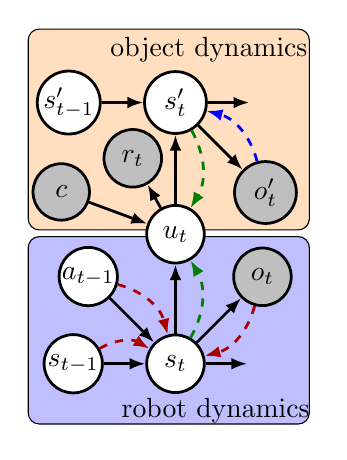
\begin{tikzpicture}[scale=0.85]
    \begin{scope}[yshift=8cm,node distance=2.5em and 1.5em]
	\path [draw, fill={rgb:blue,1;white,3}, rounded corners] (-2.2,-0.9) rectangle (2.0,1.9) {};
	\path [draw, fill={rgb:orange,1;white,3}, rounded corners] (-2.2,2.0) rectangle (2.0,5.0) {};
	\node[] (rob_dyn) at (0.6,-0.7) {robot dynamics};
	\node[] (obj_dyn) at (0.5,4.7) {object dynamics};
    \node[mystyle, fill={rgb:white,1},            ] (st) {$s_t$};
    \node[mystyle, fill={rgb:white,1}, above=of st] (ut) {$u_t$};
    \node[mystyle, fill={rgb:white,1}, above=of ut] (sts) {$s'_t$};
    \node[mystyle, fill={rgb:white,1}, left=of sts] (stsm1) {$s'_{t-1}$};
    \node[right=of sts] (stsp1) {};
    \node[mystyle, fill={rgb:black,1;white,3}, below right=1.6em and 1.6em of sts] (ots) {$o'_t$};
    \node[mystyle, fill={rgb:black,1;white,3}, above left=1.2em and 0.0em of ut] (rt) {$r_t$};
    \node[mystyle, fill={rgb:black,1;white,3}, above left=0.0em and 2.6em of ut] (c) {$c$};
    \node[mystyle, fill={rgb:white,1}, left=of st] (stm1) {$s_{t-1}$};
    \node[mystyle, fill={rgb:white,1}, above left=1.6em and 1.6em of st] (atm1) {$a_{t-1}$};
    \node[mystyle, fill={rgb:black,1;white,3}, above right=1.6em and 1.6em of st] (ot) {$o_t$};
    % \node[mystyle, fill={rgb:black,1;brown,3}, above left=0.9em and 0.1em of ut] (u1t) {$u_t$};
    \node[right=of st] (stp1) {};
    \draw[myline] (stsm1) -- (sts);
	\draw[myline] (sts) -- (stsp1);
	\draw[myline] (sts) -- (ots);
	\draw[myline] (st) -- (ut);
	\draw[myline] (ut) -- (sts);
	\draw[myline] (stm1) -- (st);
	\draw[myline] (atm1) -- (st);
	\draw[myline] (st) -- (ot);
	\draw[myline] (c) -- (ut);
	\draw[myline] (ut) -- (rt);
	\draw[myline] (st) -- (stp1);
	\draw[myline, dashed, color=blue] (ots) edge[bend right] (sts);
% 	\draw[myline, color={rgb:brown,1;black,1}] (ots) edge[bend right=20, mysnake,] (ut);
% 	\draw[myline, color={rgb:brown,1;black,1}] (st) edge[bend left=20, mysnake,] (ut);
	\draw[myline, dashed, color={rgb:green,1;black,1}] (sts) edge[bend left] (ut);
	\draw[myline, dashed, color={rgb:green,1;black,1}] (st) edge[bend right] (ut);
	
	\draw[myline, dashed, color={rgb:red,2;black,1}] (stm1) edge[bend left] (st);
	\draw[myline, dashed, color={rgb:red,2;black,1}] (atm1) edge[bend left] (st);
	\draw[myline, dashed, color={rgb:red,2;black,1}] (ot) edge[bend left] (st);
	\end{scope}
  \end{tikzpicture}
    }
    \scalebox{0.75}{
        \begin{tikzpicture}[scale=1.0]
    \begin{scope}[yshift=8cm,node distance=2.5em and 1.5em]
    \path [draw, fill={rgb:blue,1;white,3}, rounded corners] (-2.2,-0.9) rectangle (2.0,1.9) {};
    \path [draw, fill={rgb:orange,1;white,3}, rounded corners] (-2.2,2.0) rectangle (2.0,5.0) {};
    
    % robot part
	\node[] (rob_dyn) at (0.0,-0.7) {манипулятор};
    \node[mystyle, fill={rgb:white,1},            ] (st) {$s^r_t$};
    \node[mystyle, fill={rgb:white,1}, left=of st] (stm1) {$s^r_{t-1}$};
    \node[mystyle, fill={rgb:white,1}, above left=1.6em and 1.6em of st] (atm1) {$a_{t-1}$};
    \node[mystyle, fill={rgb:black,1;white,3}, above right=1.6em and 1.6em of st] (ot) {$o^r_t$};
    \node[right=of st] (stp1) {};
	
	% influence part
    \node[mystyle, fill={rgb:white,1}, above=of st] (ut) {$u_t$};
    % \node[mystyle, fill={rgb:black,1;white,3}, above left=0.5em and 1.5em of ut] (c) {$c$};
	
	% object part
	\node[] (obj_dyn) at (0.0,4.7) {объект};
    \node[mystyle, fill={rgb:white,1}] (sts) at (0.0, 3.9) {$s^o_t$};
    \node[mystyle, fill={rgb:white,1}, left=of sts] (stsm1) {$s^o_{t-1}$};
    \node[mystyle, fill={rgb:black,1;white,3}, below right=1.6em and 1.6em of sts] (ots) {$o^o_t$};
    \node[right=of sts] (stsp1) {};
    \node[mystyle, fill={rgb:black,1;white,3}, below left=1.6em and 1.6em of sts] (c) {$c$};
    
    % robot edges
	\draw[myline] (stm1) -- (st);
	\draw[myline] (atm1) -- (st);
	\draw[myline] (st) -- (stp1);
	\draw[myline] (st) -- (ot);
	
	% influence edges
	\draw[myline] (st) -- (ut);
	\draw[myline] (ut) -- (sts);
	\draw[myline] (c) -- (ut);
	
	% object edges
    \draw[myline] (stsm1) -- (sts);
	\draw[myline] (sts) -- (stsp1);
	\draw[myline] (sts) -- (ots);
	
	% inference edges
	\draw[myline, dashed, color={rgb:green,1;black,1}] (sts) edge[bend left] (ut);
	\draw[myline, dashed, color={rgb:green,1;black,1}] (st) edge[bend right] (ut);
	\end{scope}
  \end{tikzpicture}
    }
    \scalebox{0.75}{
        \begin{tikzpicture}[scale=1.0]
    \begin{scope}[yshift=8cm,node distance=2.5em and 1.5em]
    \path [draw, fill={rgb:blue,1;white,3}, rounded corners] (-2.2,-0.9) rectangle (2.0,1.9) {};
    \path [draw, fill={rgb:orange,1;white,3}, rounded corners] (-2.2,2.0) rectangle (2.0,5.0) {};
    
    % robot part
	\node[] (rob_dyn) at (0.0,-0.7) {манипулятор};
    \node[mystyle, fill={rgb:white,1},            ] (st) {$s^r_t$};
    \node[mystyle, fill={rgb:white,1}, left=of st] (stm1) {$s^r_{t-1}$};
    \node[mystyle, fill={rgb:white,1}, above left=1.6em and 1.6em of st] (atm1) {$a_{t-1}$};
    \node[mystyle, fill={rgb:black,1;white,3}, above right=1.6em and 1.6em of st] (ot) {$o^r_t$};
    \node[right=of st] (stp1) {};
	
	% influence part
    \node[mystyle, fill={rgb:white,1}, above=of st] (ut) {$u_t$};
    % \node[mystyle, fill={rgb:black,1;white,3}, above left=0.5em and 1.5em of ut] (c) {$c$};
	
	% object part
	\node[] (obj_dyn) at (0.0,4.7) {объект};
    \node[mystyle, fill={rgb:white,1}] (sts) at (0.0, 3.9) {$s^o_t$};
    \node[mystyle, fill={rgb:white,1}, left=of sts] (stsm1) {$s^o_{t-1}$};
    \node[mystyle, fill={rgb:black,1;white,3}, below right=1.6em and 1.6em of sts] (ots) {$o^o_t$};
    \node[right=of sts] (stsp1) {};
    % \node[mystyle, fill={rgb:black,1;white,3}, below left=1.6em and 1.6em of sts] (c) {$c$};
    
    % robot edges
	\draw[myline] (stm1) -- (st);
	\draw[myline] (atm1) -- (st);
	\draw[myline] (st) -- (stp1);
	\draw[myline] (st) -- (ot);
	
	% influence edges
	\draw[myline] (st) -- (ut);
	\draw[myline] (ut) -- (sts);
% 	\draw[myline] (c) -- (ut);
	
	% object edges
    \draw[myline] (stsm1) -- (sts);
	\draw[myline] (sts) -- (stsp1);
	\draw[myline] (sts) -- (ots);
	
	% inference edges
	\draw[myline, dashed, color={rgb:green,1;black,1}] (sts) edge[bend left] (ut);
	\draw[myline, dashed, color={rgb:green,1;black,1}] (st) edge[bend right] (ut);
	\end{scope}
  \end{tikzpicture}
    }
    \caption{Предлагаемые архитектуры}
    \label{fig:archs}
\end{figure}

Проверенные в ходе исследования модели алгоритмов изображены графически на рис. \ref{fig:archs}.
Для удобства описания, алгоритмы, использующие факторизованные модели мира, приведены под названием CEMA (Cause-Effect Modeling Agent).
Таким образом, наиболее уместными выглядят следующие модели:
\begin{itemize}
    \item \textbf{CEMA-Direct}: Модель мира прямого влияния \ref{eq:instant}, $\pi(a_t \mid s^r_t, s^o_t, c)$, $\nu(s^r_t, s^o_t)$, $r(s^o_t)$
    \item \textbf{CEMA-TopDown}: Модель мира косвенного влияния \ref{eq:cema-td}, однозадачный вектор влияния, $\pi(a_t \mid s^r_t, s^o_t, u_t)$, $\nu(s^r_t, s^o_t, u_t)$, $r(u_t)$
    \item \textbf{CEMA-Influence}: Модель мира косвенного влияния \ref{eq:cema-infl}, однозадачный вектор влияния, $\pi(a_t \mid s^r_t, s^o_t, u_t)$, $\nu(s^r_t, s^o_t, u_t)$, $r(u_t)$
    \item \textbf{CEMA-Generalize}: Модель мира косвенного влияния \ref{eq:cema-infl}, многозадачный вектор влияния, $\pi(a_t \mid s^r_t, s^o_t, u_t, c)$, $\nu(s^r_t, s^o_t)$, $r(s^o_t, u_t)$ 
\end{itemize}




\clearpage
%%%%%%%%%%%%%%%%%%%%%%%%%%%%%%%%%%%%%%%%%%%%%%%%%%%%%%%%%%%%%%%%%%%%%%%%%%
\section{Вычислительные эксперименты}
%%%%%%%%%%%%%%%%%%%%%%%%%%%%%%%%%%%%%%%%%%%%%%%%%%%%%%%%%%%%%%%%%%%%%%%%%%

% Описывается прикладная задача,
% параметры анализируемых данных (например, сколько объектов, сколько признаков, каких они типов),
% параметры эксперимента (например, как генерировались модельные данные, как производился скользящий контроль).
% Результаты экспериментов представляются в~виде таблиц и~графиков.
% Объясняется точный смысл всех обозначений на~графиках, строк и~столбцов в~таблицах.
% Приводятся выводы:
% в~какой степени результаты экспериментов согласуются с теорией?
% Достигнут ли желаемый результат?
% Обнаружены ли какие-либо факты, не~нашедшие объяснения,
% и~которые нельзя списать на «грязный» эксперимент?

% Цель данного раздела:
% продемонстрировать, что предложенная теория работает на практике;
% показать границы её применимости;
% рассказать о~новых экспериментальных фактах.

% Чисто теоретические работы могут не содержать данного раздела (на~практике не~работает, ну и~не~надо "--- зато теория красивая).
% Кстати, теоретики имеют право не догадываться, где, кому и~когда их~теории пригодятся.

Тестирование моделей мира проводилось в двух бенчмарках обучения с подкрепления, MetaWorld \cite{mtw} и CasualWorld \cite{cw}. 
Оба пакета предоставляют инструментарий для разработки и тестирования сред и алгоритмов обучения с подкреплениями, решающих задачу роботизированного контроля.

\subsection{Эксперименты в наборе сред MetaWorld}
Библиотека сред MetaWorld \cite{mtw} предоставляет широкие возможности для тестирования и сравнения алгоритмов мета-обучения и мультизадачного обучения и состоит из 50 задач, различающихся объектами, присутствующими в среде и целями, которые алгоритм должен достичь. Предлагаемые в работе архитектуры моделей мира в первую очередь рассчитаны на обобщение между задачами, имеющими одинаковую семантическую структуру, поэтому проверка алгоритма на всем наборе представляется неуместной. Также, некоторые из задач являются достаточно сложными даже для базового алгоритма, что представляло бы трудности в анализе обобщающей способности.

Для удобного тестирования предложенного подхода была создана новая среда, предлагаемое название которой RotatedDrawerOpen.
В ней содержится два объекта - шкаф с выдвижным ящиком и робот.
В конкретной задаче позиция шкафа закреплена, однако между задачами она меняется.
Примеры изображений различных задач среды представлены на рисунке \ref{fig:rdw}.

\begin{figure}[h]
    \centering
    \begin{subfigure}{.3\textwidth}
        \centering
        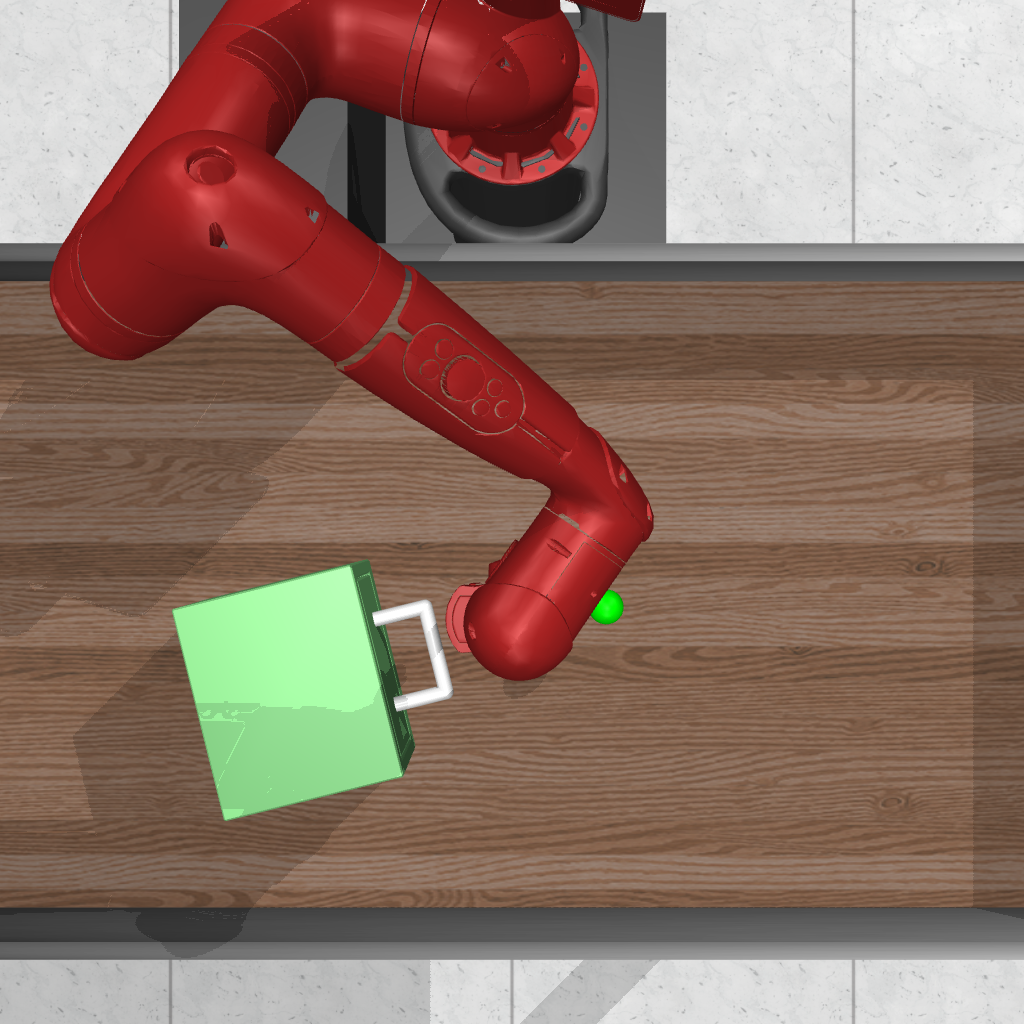
\includegraphics[width=\linewidth]{figures/pos1.png}
    \end{subfigure}
    \begin{subfigure}{.3\textwidth}
        \centering
        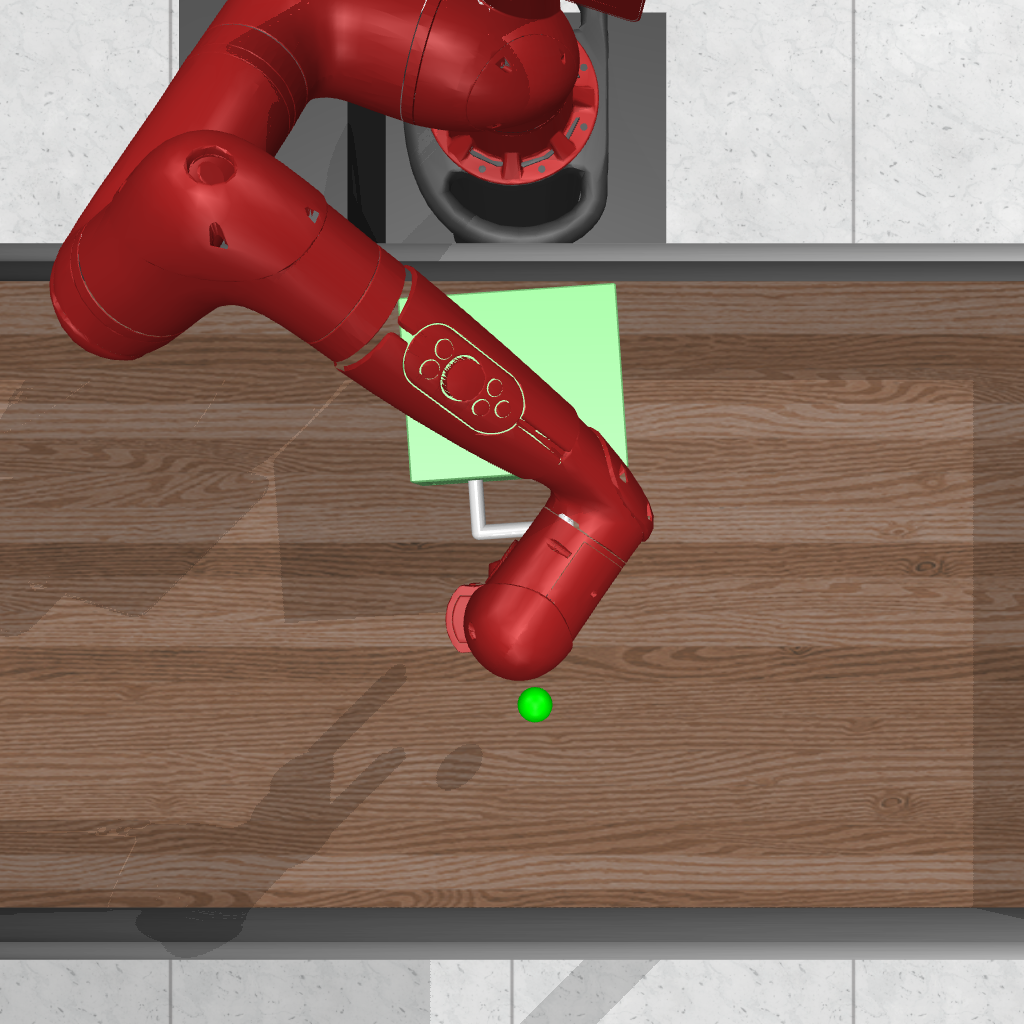
\includegraphics[width=\linewidth]{figures/pos2.png}
    \end{subfigure}
    \begin{subfigure}{.3\textwidth}
        \centering
        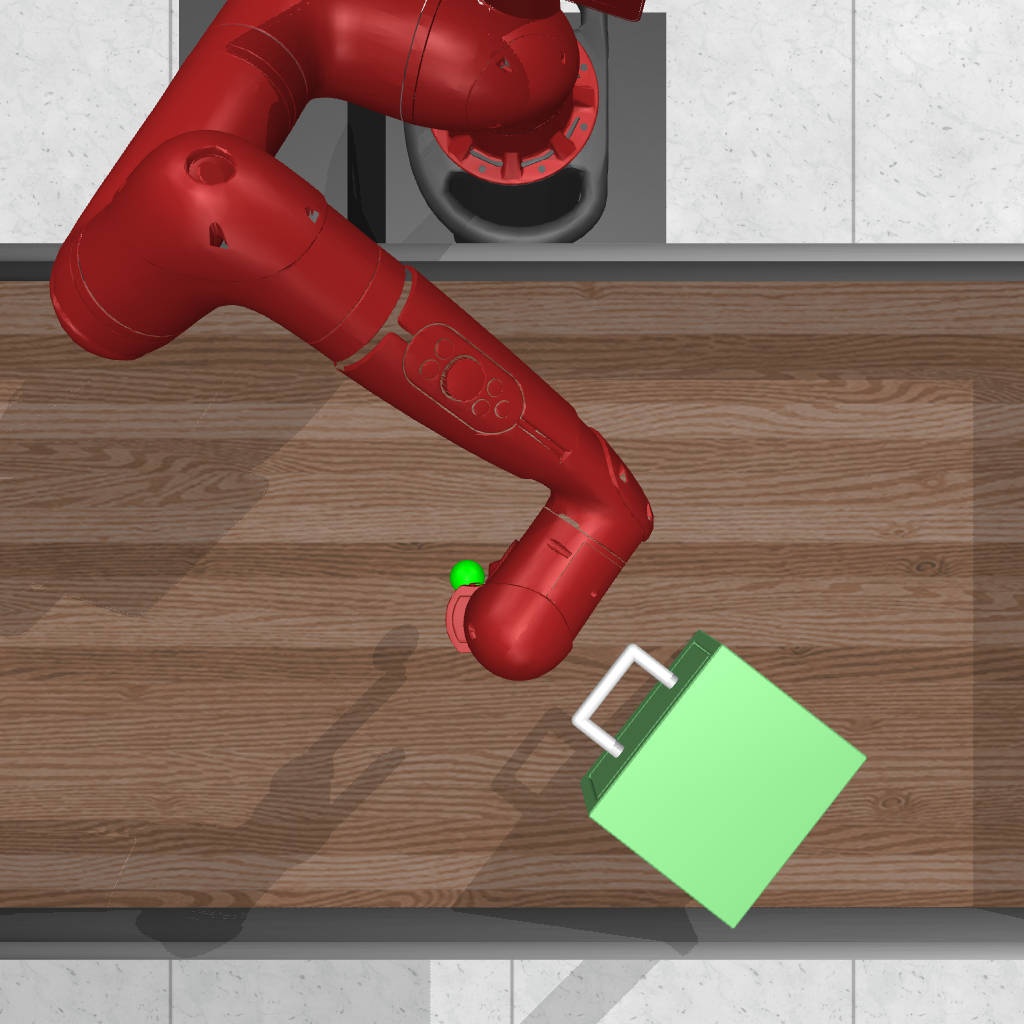
\includegraphics[width=\linewidth]{figures/pos3.png}
    \end{subfigure}
    \caption{Примеры задач в среде RotatedDrawerOpen.}
    \label{fig:rdw}
\end{figure}

Рассмотрим полярную систему координат с центром в середине сцены, в ней центр ящика имеет координаты $(R, \alpha_{\tau}, h)$.
Для всех задач значения координат $R$ и $h$ одинаковы и не меняются ни в течения эпизода, ни между задачами.
Множество задач, таким образом, совпадает с множеством значений $\alpha_{\tau}$ и равно $\left[0, 2\pi\right) \in \mathbb{R}$.
Контекст $c$ в экспериментах в этой среде определяется следующим образом:
\begin{equation}
    c = \alpha_{\tau}, \quad \forall{\tau} \in \mathcal{T}
\end{equation}
Множество задач $\mathcal{T}$ разделено на $\mathcal{T}_{\text{train}}$ и $\mathcal{T}_{\text{test}}$ следующим образом:
\begin{align}
    \mathcal{T}_{\text{train}} = & \{\tau \mid 
    \alpha_{\tau} \in \left[0, \frac{\pi}{4}\right) \cup \left[\frac{3\pi}{4}, \frac{5\pi}{4}\right) \cup
    \left[\frac{7\pi}{4}, 2\pi\right)\};
    \notag
    \\
    \mathcal{T}_{\text{test}} = & \{\tau \mid \alpha_{\tau} \in \left[\frac{\pi}{4}, \frac{3\pi}{4}\right) \cup \left[\frac{5\pi}{4}, \frac{7\pi}{4}\right)\}.
\end{align}
Разделение такого вида выбрано для уменьшения эффекта ухудшения работы энкодера на изображениях с еще не виденной позицией шкафа.
Действия $a \in \mathbb{R}^4$ представляют собой координаты следующего положения руки робота и число, регулирующее сжатие его пальцев.

На шаге $t$ агент получает получает из среды в качестве наблюдения робота $o_t$ и наблюдения объекта $o'_t$ сегментированные изображения робота и объекта соответственно.
Изображения являются тензорами размера $64 \times 64 \times 3$, камера для всех задач зафиксирована в одном положении сверху сцены.
Из-за подобного расположения камеры, сегментационная маска шкафа достаточно часто перекрыта изображением робота, в особенности в процессе выдвижения ящика.
Тогда как подобная ситуация вписывается в постановку задачи и должна решаться алгоритмом за счет рекуррентного вывода $q(s^o_{t+1} \mid s^o_{t}, u_t, o^o_{t+1})$, визуальные дефекты маски объекта могут мешать обучению объектной части модели мира, в особенности если вывод не рекуррентен $q(s^o_{t+1} \mid o^o_{t+1})$.
Чтобы исключить из анализа этот эффект, среда предоставляет в качестве объектного наблюдения $o^o_t$ сегментационную маску объекта, полученную из виртуальной копии среды без робота.
Функция награды не является разреженной и полностью соответствует функции награды из среды DrawerOpen пакета MetaWorld.

Подобная среда была выбрана для экспериментирования по нескольким причинам:
\begin{itemize}
    \item Каждая отдельная задача в среде является достаточно простой для базового алгоритма, что позволяет сфокусироваться на улучшении обобщающей способности без необходимости проводить долгий процесс обучения и модификации алгоритма под задачу.
    \item Все задачи в среде имеют одну и ту же структуру, зависящую от единственного параметра вариации, что делает полученные результаты более визуализируемыми и трактуемыми.
    \item Структура задач в среде позволяет алгоритму получить достаточно информации из единственной камеры с закрепленным положением, что избавляет агента от необходимости обрабатывать сложные 3-D композиции положений объекта.
\end{itemize}

\begin{figure}[t]
    \centering
    \begin{subfigure}{.47\textwidth}
        \centering
        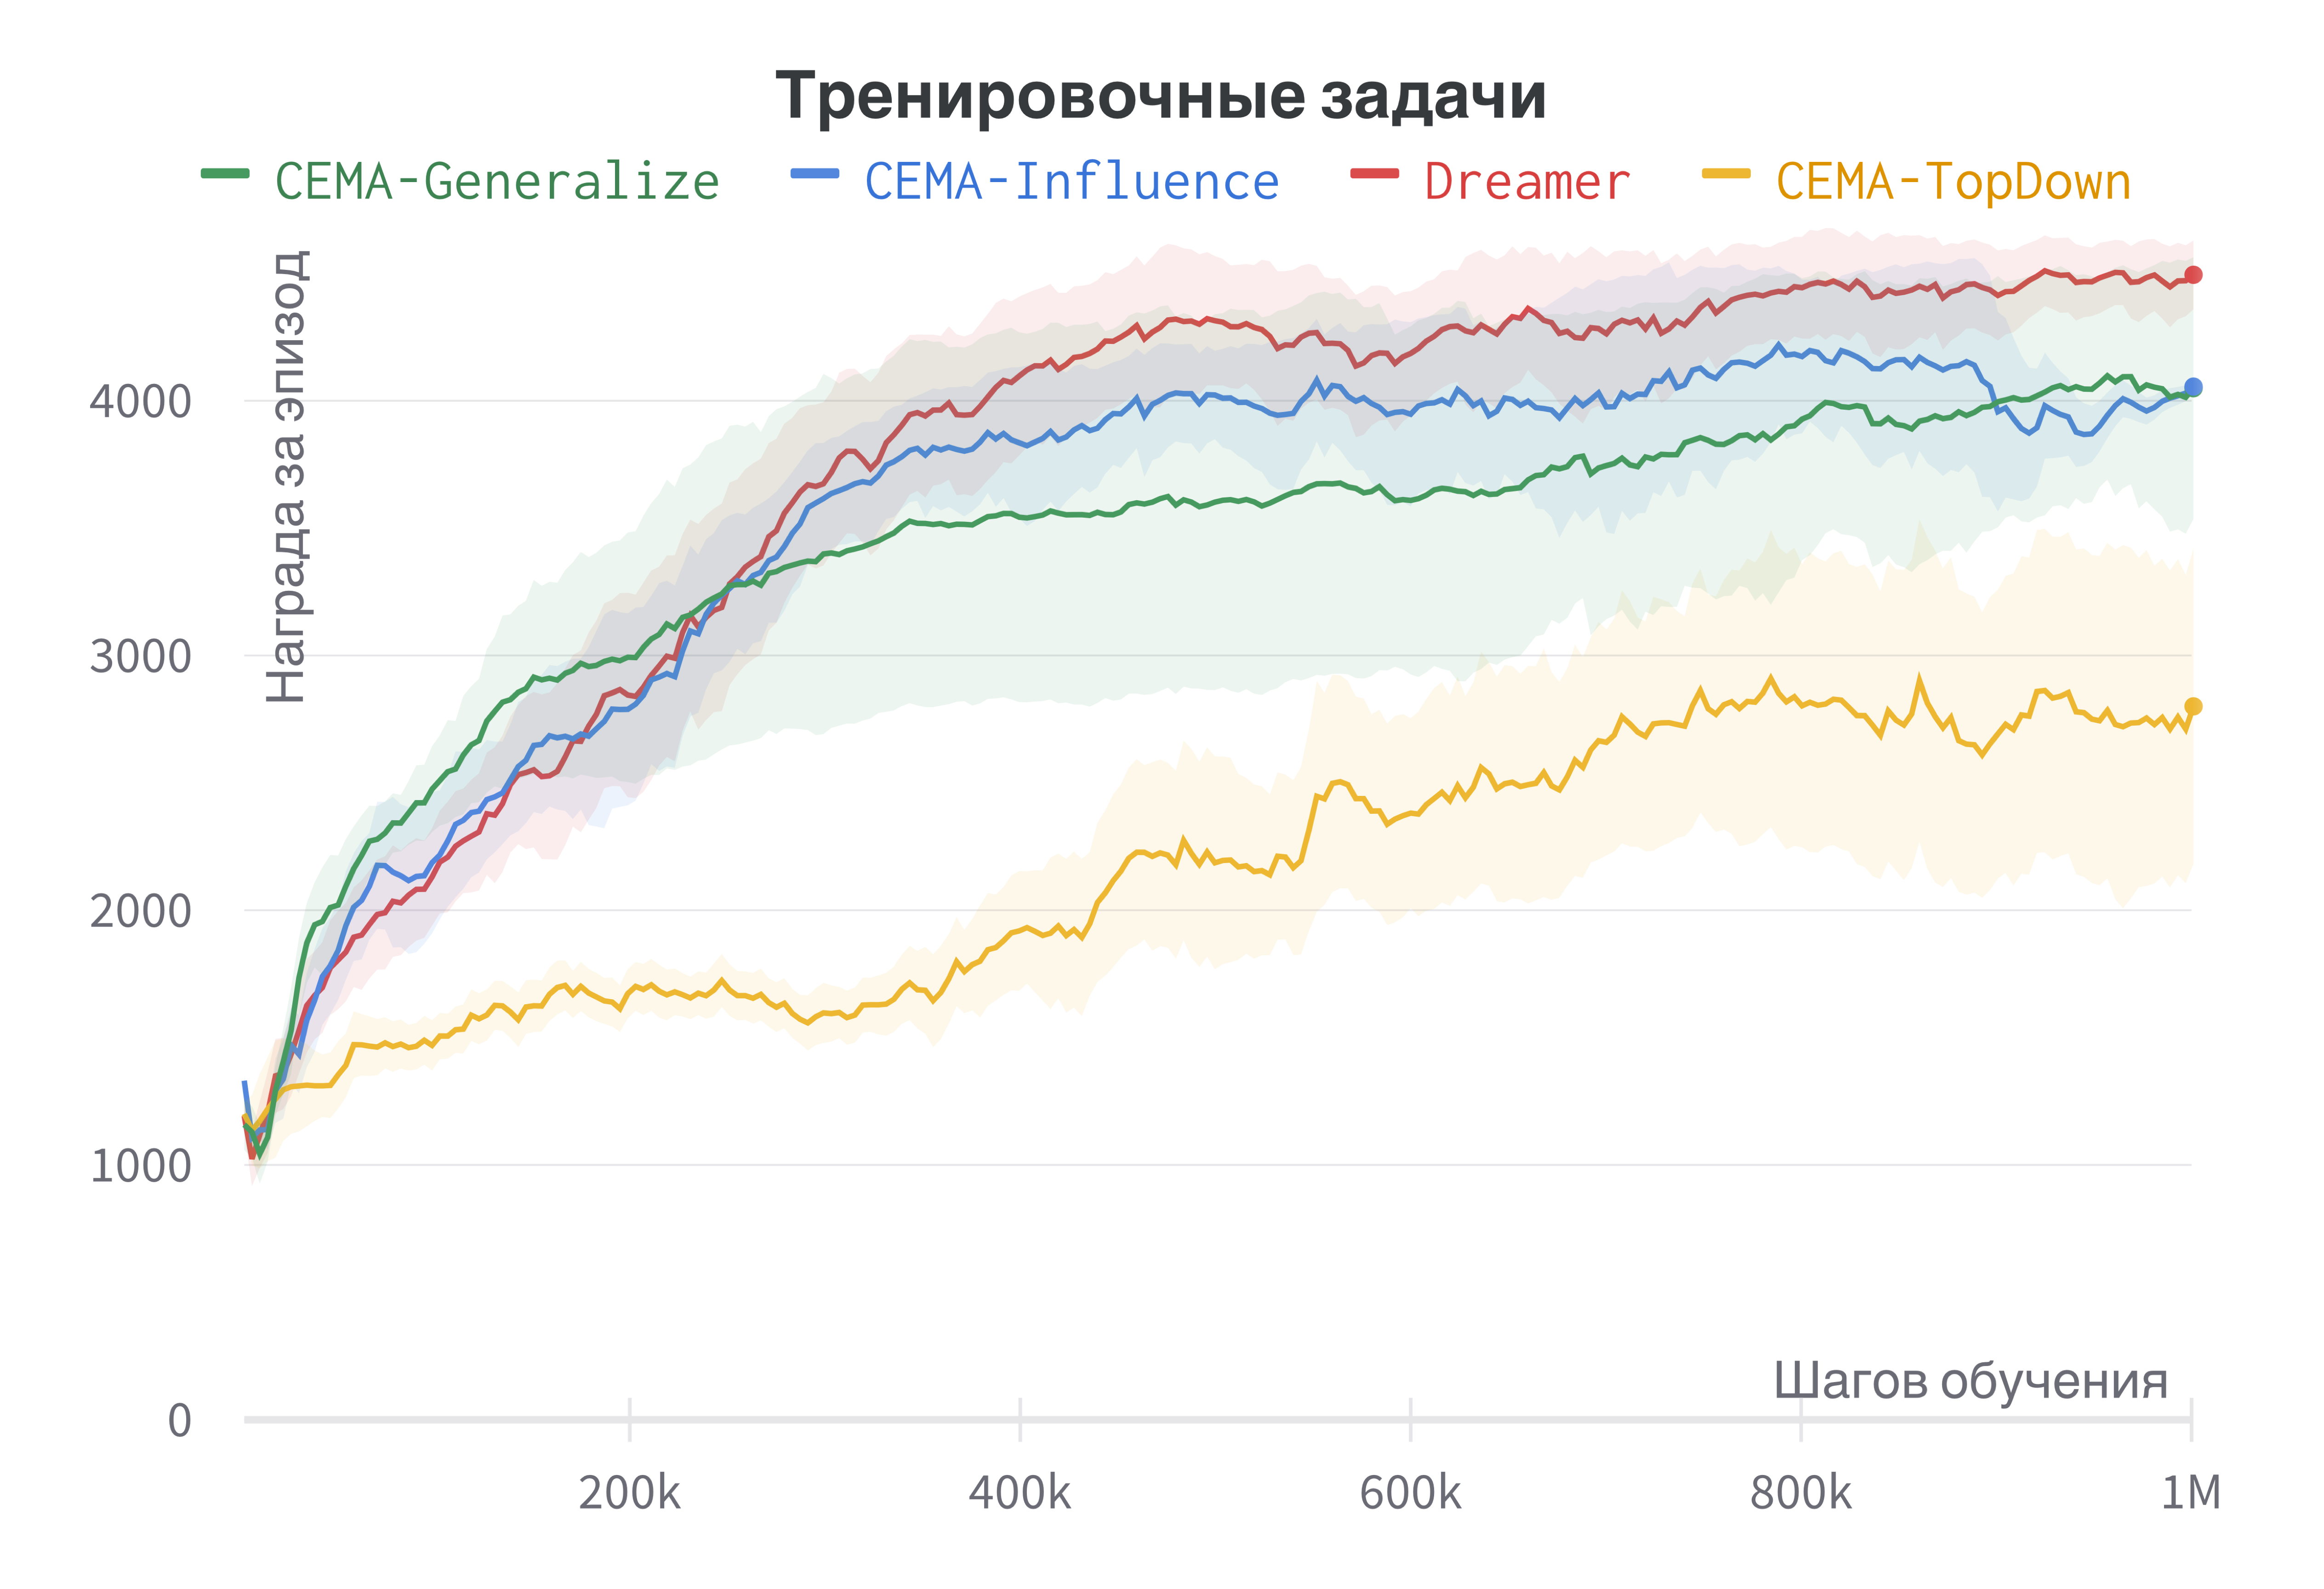
\includegraphics[width=\linewidth]{figures/rdw_train.png}
    \end{subfigure}
    \begin{subfigure}{.47\textwidth}
        \centering
        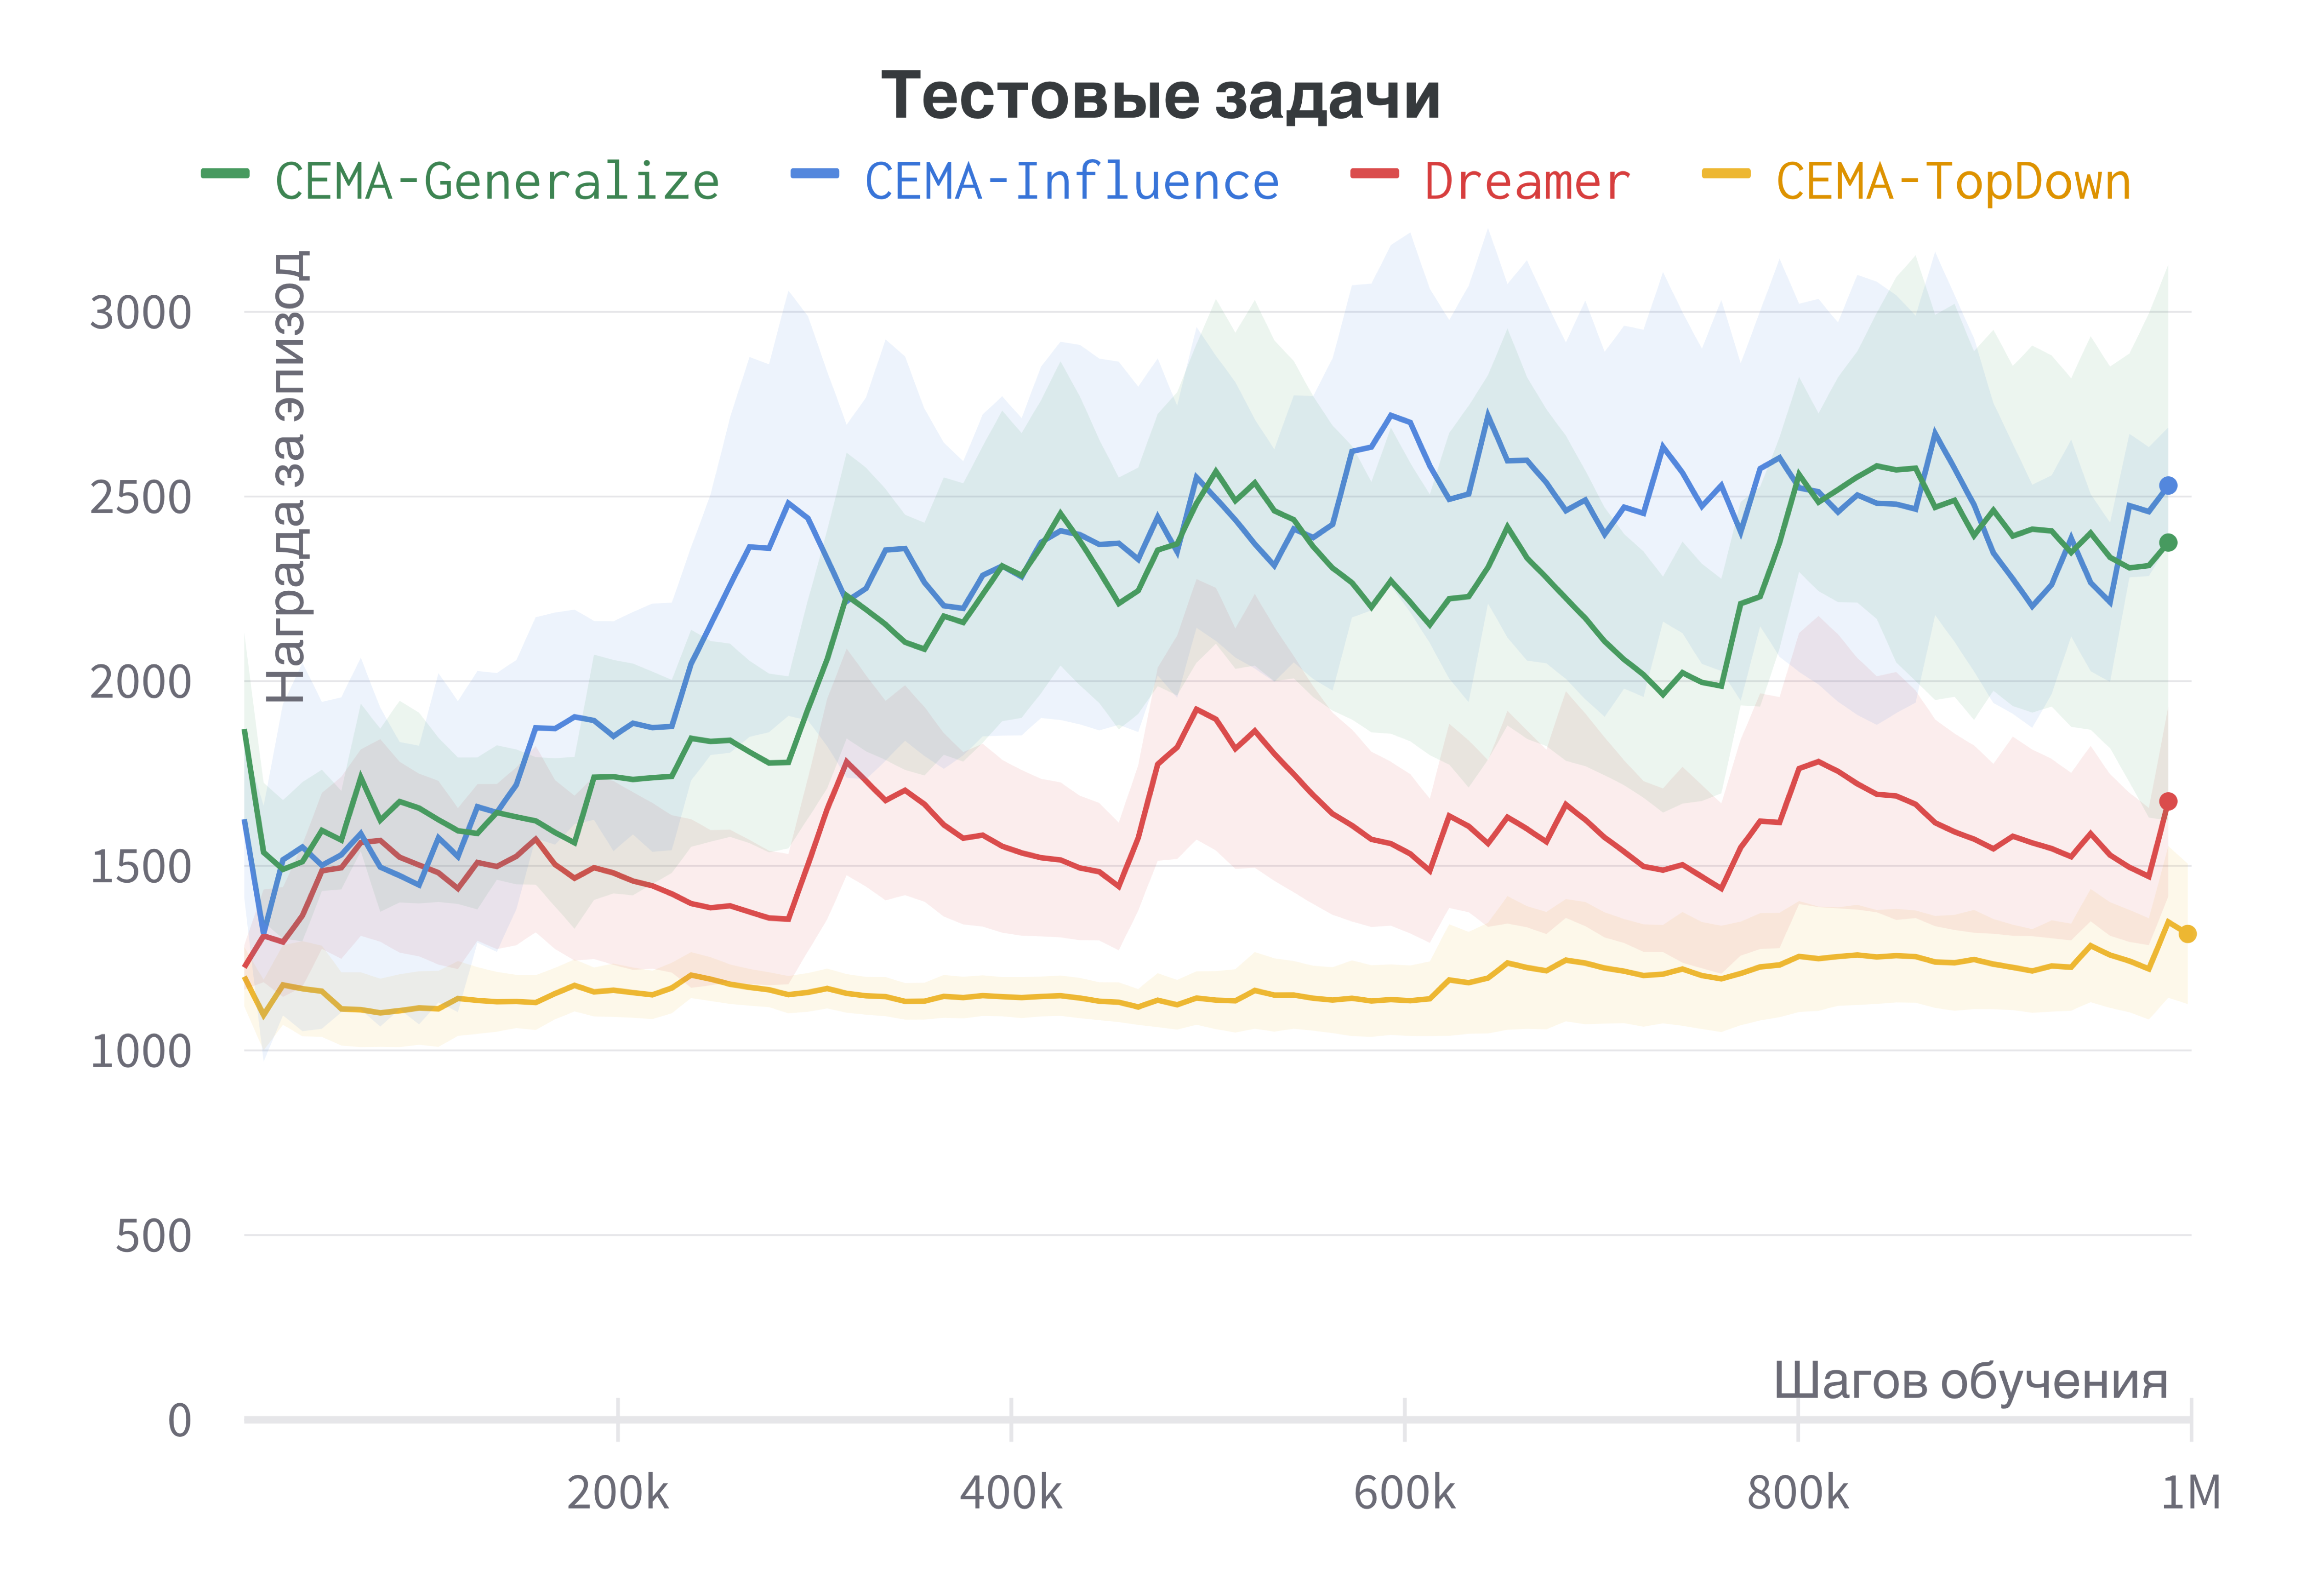
\includegraphics[width=\linewidth]{figures/rdw_test.png}
    \end{subfigure}
    \caption{Графики тренировочного процесса в среде RotatedDrawerOpen.}
    \label{fig:rdw_res}
\end{figure}

На рис. \ref{fig:rdw_res} представлены результаты обучения алгоритмов в среде RotatedDrawerOpen.
Из результатов можно заключить, что опасения, высказанные насчет варианта алгоритма CEMA-TopDown, были справедливы - даже на тренировочных задачах алгоритм показывает себя хуже остальных.
Все предложенные варианты проигрывают базовому алгоритму по скорости обучения на тренировочных задачах.
Однако важно заметить, что для вариантов CEMA-Influence и CEMA-Generalize этот проигрыш не является серьезным - награды в районе $\sim3000$ указывают на то, что алгоритм научился решать задачу, из чего следует что предложенные алгоритмы проигрывают только в скорости решения задач в конкретном эпизоде и при этом алгоритмы выходят по результатам обучения на схожую среднюю награду за эпизод.
Однако на тестовых задачах, два упомянутых алгоритма уверенно превосходят базовый, хоть их результаты и не являются устойчивыми.

\subsection{Эксперименты в наборе сред CasualWorld}
В наборе сред CasualWorld\cite{cw} представлен удобный инструментарий для оценки обобщающих способностей алгоритмов обучения с подкреплением.
Главным преимуществом по сравнению с другими библиотеками для тестирования является удобный интерфейс для параметрического изменения характеристик среды, как визуальных, так и физических.
Аналогично MetaWorld, в CasualWorld содержится набор заранее сконструированных сред и задач в них, а также заранее заданные наборы параметров варьирования задач для тренировки и тестирования алгоритмов.
Сами задачи являются более сложными по сравнению с MetaWorld из-за большей размерности пространства действий, обусловленной конструкцией манипулятора.
Эксперименты в данной среде преследовали цель проверки работы алгоритма в более близких условиях к реальным.

В качестве среды для тестирования была выбрана Pushing.
В наборе задач в этой среде от агента требуется совместить незакреплённый параллелепипед с целью такого же размера, присутствующей на изображении с камер.
Действия являются $9$-мерными векторами $a_t \in \mathbb{R}^9$ и представляют собой координаты трёх пальцев.
Для получения наблюдений используются две камеры, положение и ориентация которых закреплены для всех задач.
Каждая камера предоставляет маску сегментации для манипулятора и объекта, после чего изображения фильтруются, конкатенируются и подаются на вход как $o^r_t$ и $o^o_t$ соответственно.
Каждое получившееся наблюдение является тензором $64 \times 64 \times 6$.
Примеры отдельных изображений среды представлены на рис. \ref{fig:cw}.

\begin{figure}[t]
    \centering
    \begin{subfigure}{.3\textwidth}
        \centering
        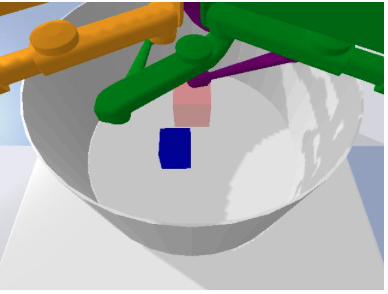
\includegraphics[width=\linewidth]{figures/obs_1.png}
    \end{subfigure}
    \begin{subfigure}{.3\textwidth}
        \centering
        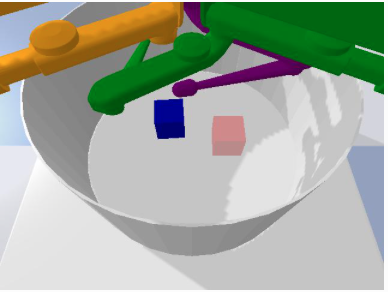
\includegraphics[width=\linewidth]{figures/obs_2.png}
    \end{subfigure}
    \begin{subfigure}{.3\textwidth}
        \centering
        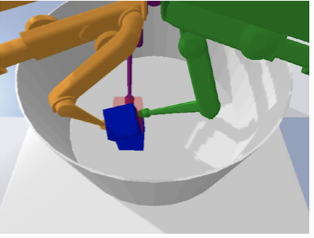
\includegraphics[width=\linewidth]{figures/obs_3.png}
    \end{subfigure}
    \caption{Примеры наблюдений в среде Pushing библиотеки CasualWorld.}
    \label{fig:cw}
\end{figure}

Встроенная функция награды является относительной, то есть зависит от предыдущего состояния среды $\mathcal{R}\left(s_t, s_{t+1}\right)$. 
Поскольку модель функции награды имеет вид $q\left(r_t \mid s_t\right)$, для базового алгоритма задача является достаточно сложной, что выражается в отсутствии прироста показателей качества модели достаточно долгое время при обучении.
Для решения данной проблемы функция награды среды была изменена.
Тогда как механика расчета наград, генерируемых средой, была оставлена нетронутой, агент наблюдает не исходные награды, а сумму всех наград с начала эпизода.
Подобный дизайн награды помогает сделать её менее зависимой от $s_t$, хотя и оставляет зависимость от начального состояния среды $s_0$.
Все представленные результаты для данной среды получены при помощи замены исходных наград $r_t$ на аккумулированные $\hat{r}_t$ в процессе обучения.

В экспериментах используются следующие вариации параметров среды:
\begin{itemize}
    \item Начальное положение объекта $\left(R_{\tau}, \alpha_{\tau}, \frac{h_{\tau}}{2}\right)$
    \item Начальная ориентация объекта $\left(R_{\tau}, \alpha_{\tau}, \frac{h_{\tau}}{2}\right)$
    \item Линейные размеры объекта $\left(l_{\tau}, w_{\tau}, h_{\tau}\right)$
    \item Масса объекта $m_{\tau}$
\end{itemize}
Подробное описание параметров вариации представлено в Таблице \ref{tbl:cw_task_spaces}.

\begin{table}[t]%\small
    \caption{Определение параметров вариации задач в CasualWorld.}
    \label{tbl:cw_task_spaces}
    \centering\medskip%\tabcolsep=2pt%\small
    \begin{tabular}{lrrr}
    \headline
        Параметр вариации
            & \multicolumn{1}{c}{Тренировочные задачи}
            & \multicolumn{1}{c}{Тестовые задачи} \\
    \headline
        {\tt Положение объекта}
            & от $[0.0, - \pi, 0.425]$ & до $[0.11, - \pi, 0.425]$ \\
            & до $[0.11, \pi, 0.425]$ & до $[0.15, \pi, 0.425]$ \\
        {\tt Ориентация объекта}
            & от $[0, 0, -\pi]$ & от $[0, 0, -\pi]$ \\
            & до $[0, 0, \pi]$ & до $[0, 0, \pi]$ \\
        {\tt Размеры объекта}
            & от $[0.075, 0.075, 0.085]$ & от $[0.095, 0.095, 0.085]$ \\
            & до $[0.095, 0.095, 0.085]$ & до $[0.115, 0.115, 0.085]$ \\
        {\tt Масса объекта}
            & от $0.015$ & от $0.045$ \\
            & до $0.045$ & до $0.10$ \\
    \hline
    \end{tabular}
\end{table}

На рис. \ref{fig:cw_res} представлены результаты обучения алгоритмов в среде CasualWorld.
После результатов, полученных на эксперименте в RotatedDrawerWorld, было принято решение исключить более слабый алгоритм CEMA-TopDown из числа рассматриваемых по причине большей сложности CasualWorld.
Как можно заключить из графиков, все испытанные методы уверенно превосходят базовый алгоритм на тренировочных задачах.
На тестовых задачах вариант CEMA-Generalize показывает себя хуже, что может быть проявлением усложнившегося взаимодействия с объектом - вектору влияния слишком сложно предсказать все варианты того, как манипулятор может влиять на объект в любой момент времени.

\begin{figure}[t]
    \centering
    \begin{subfigure}{.47\textwidth}
        \centering
        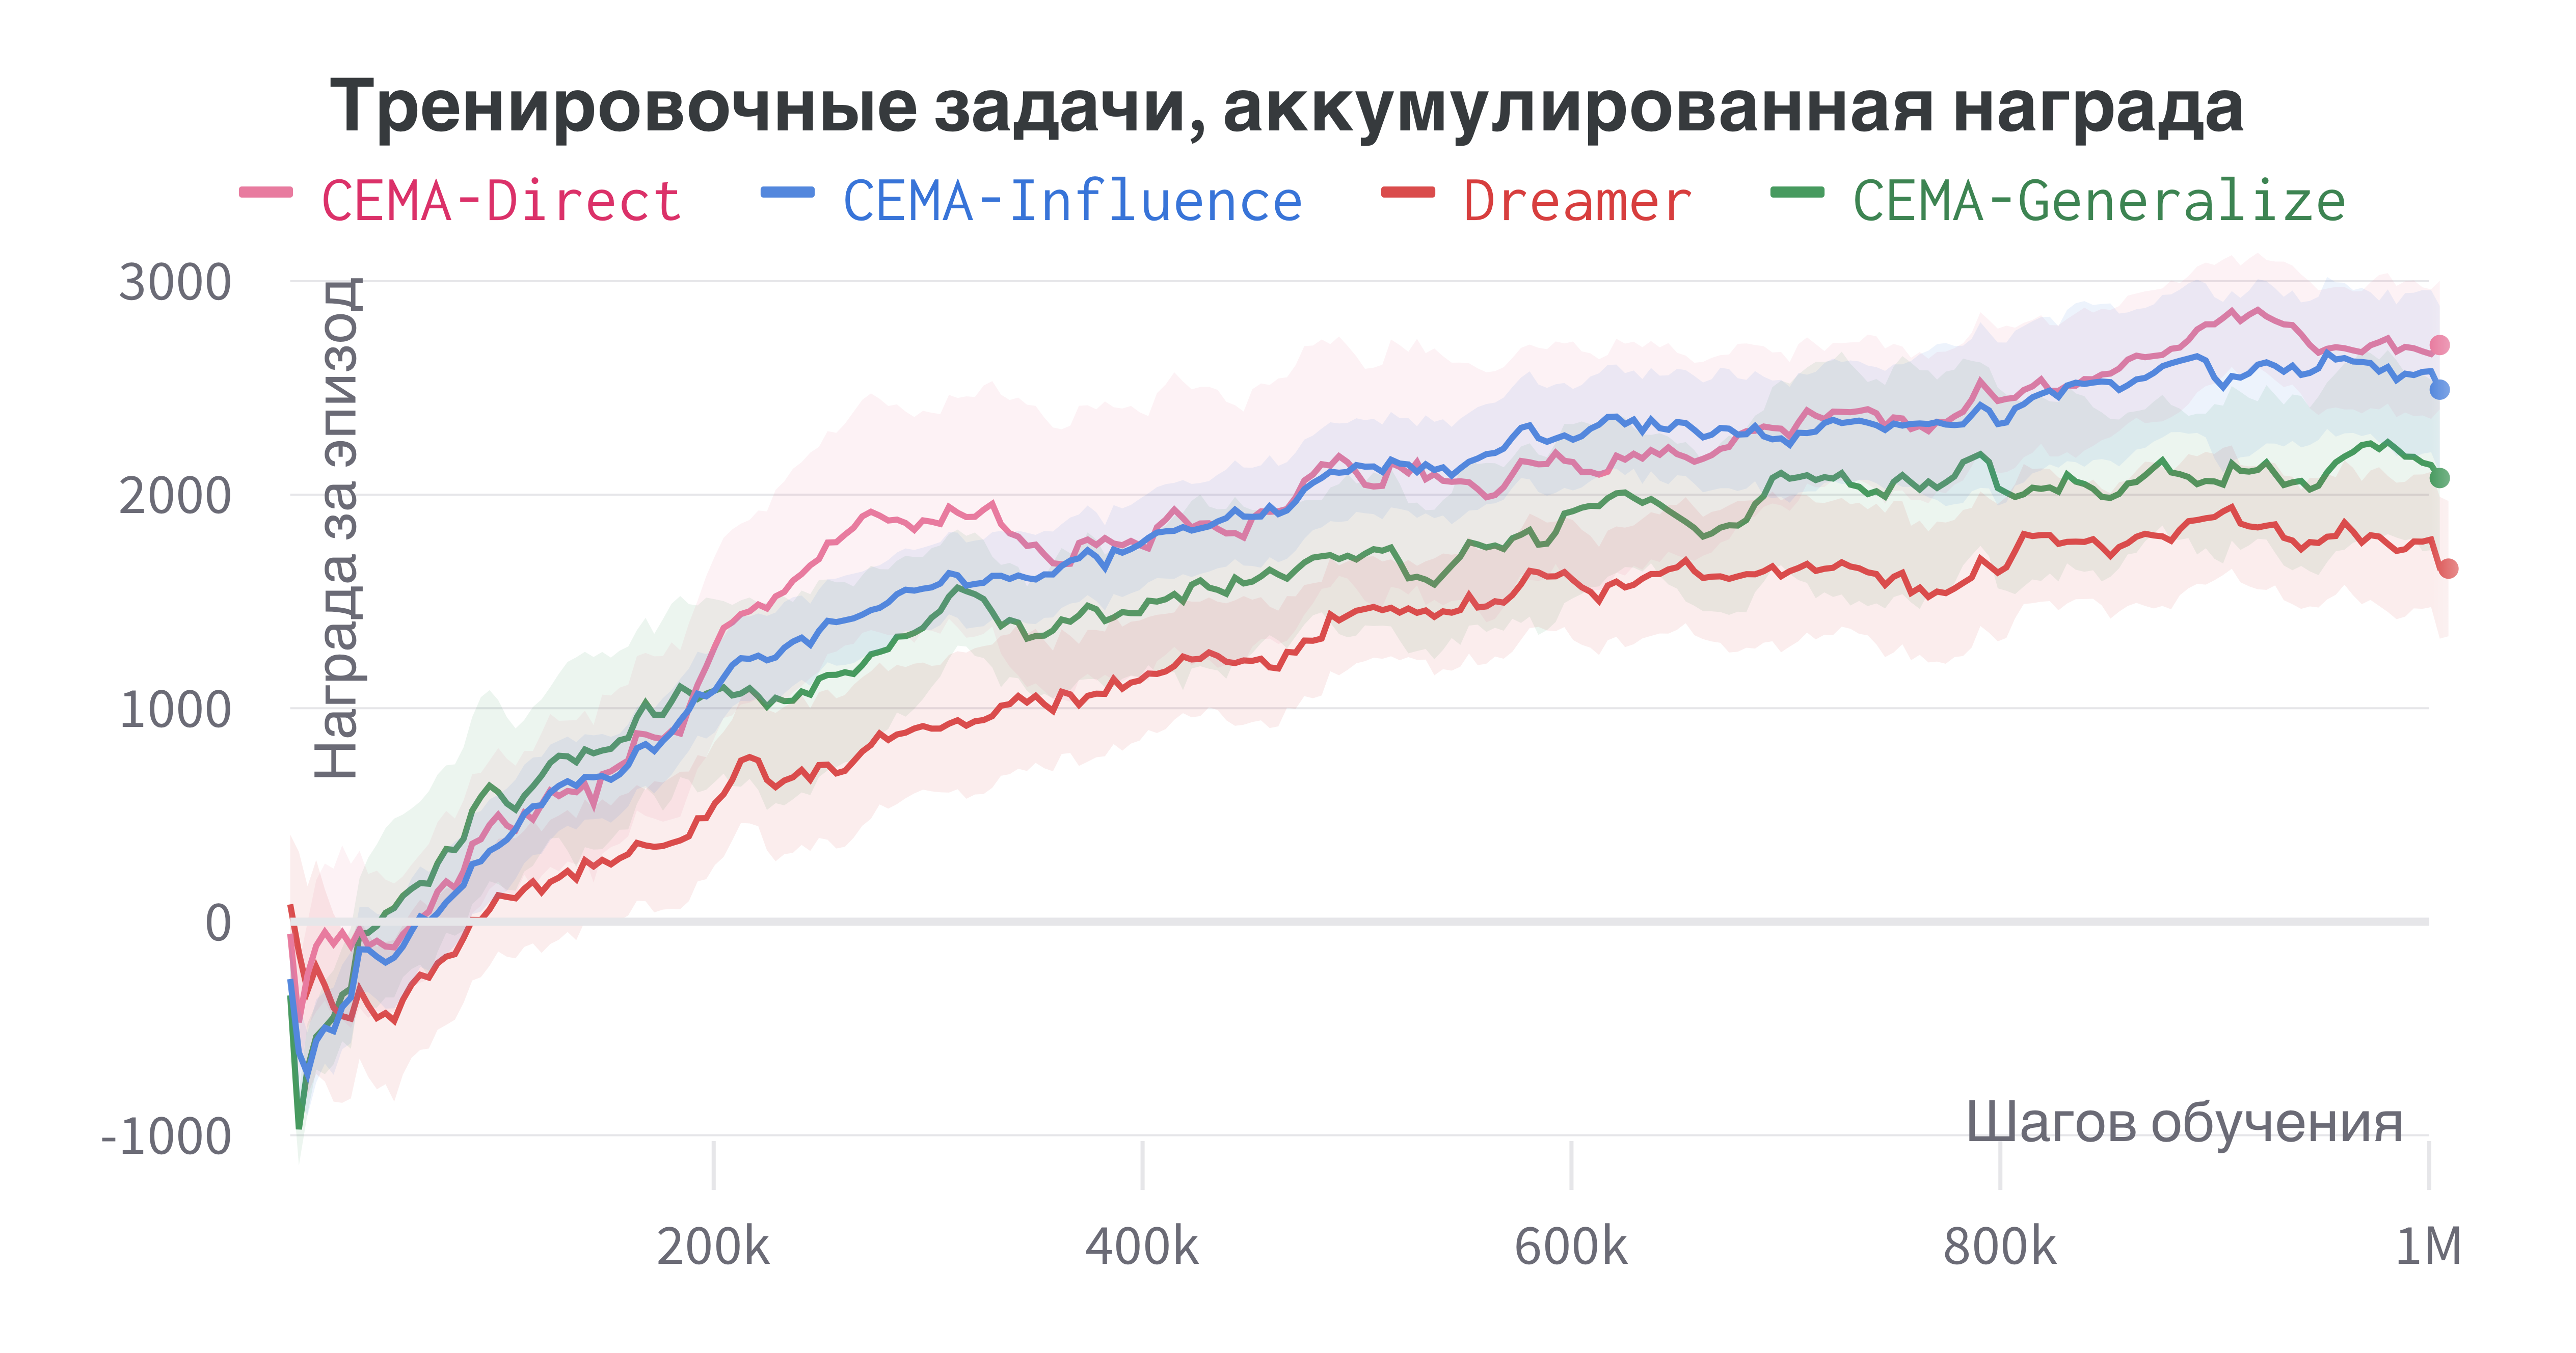
\includegraphics[width=\linewidth]{figures/cw_cum_train.png}
        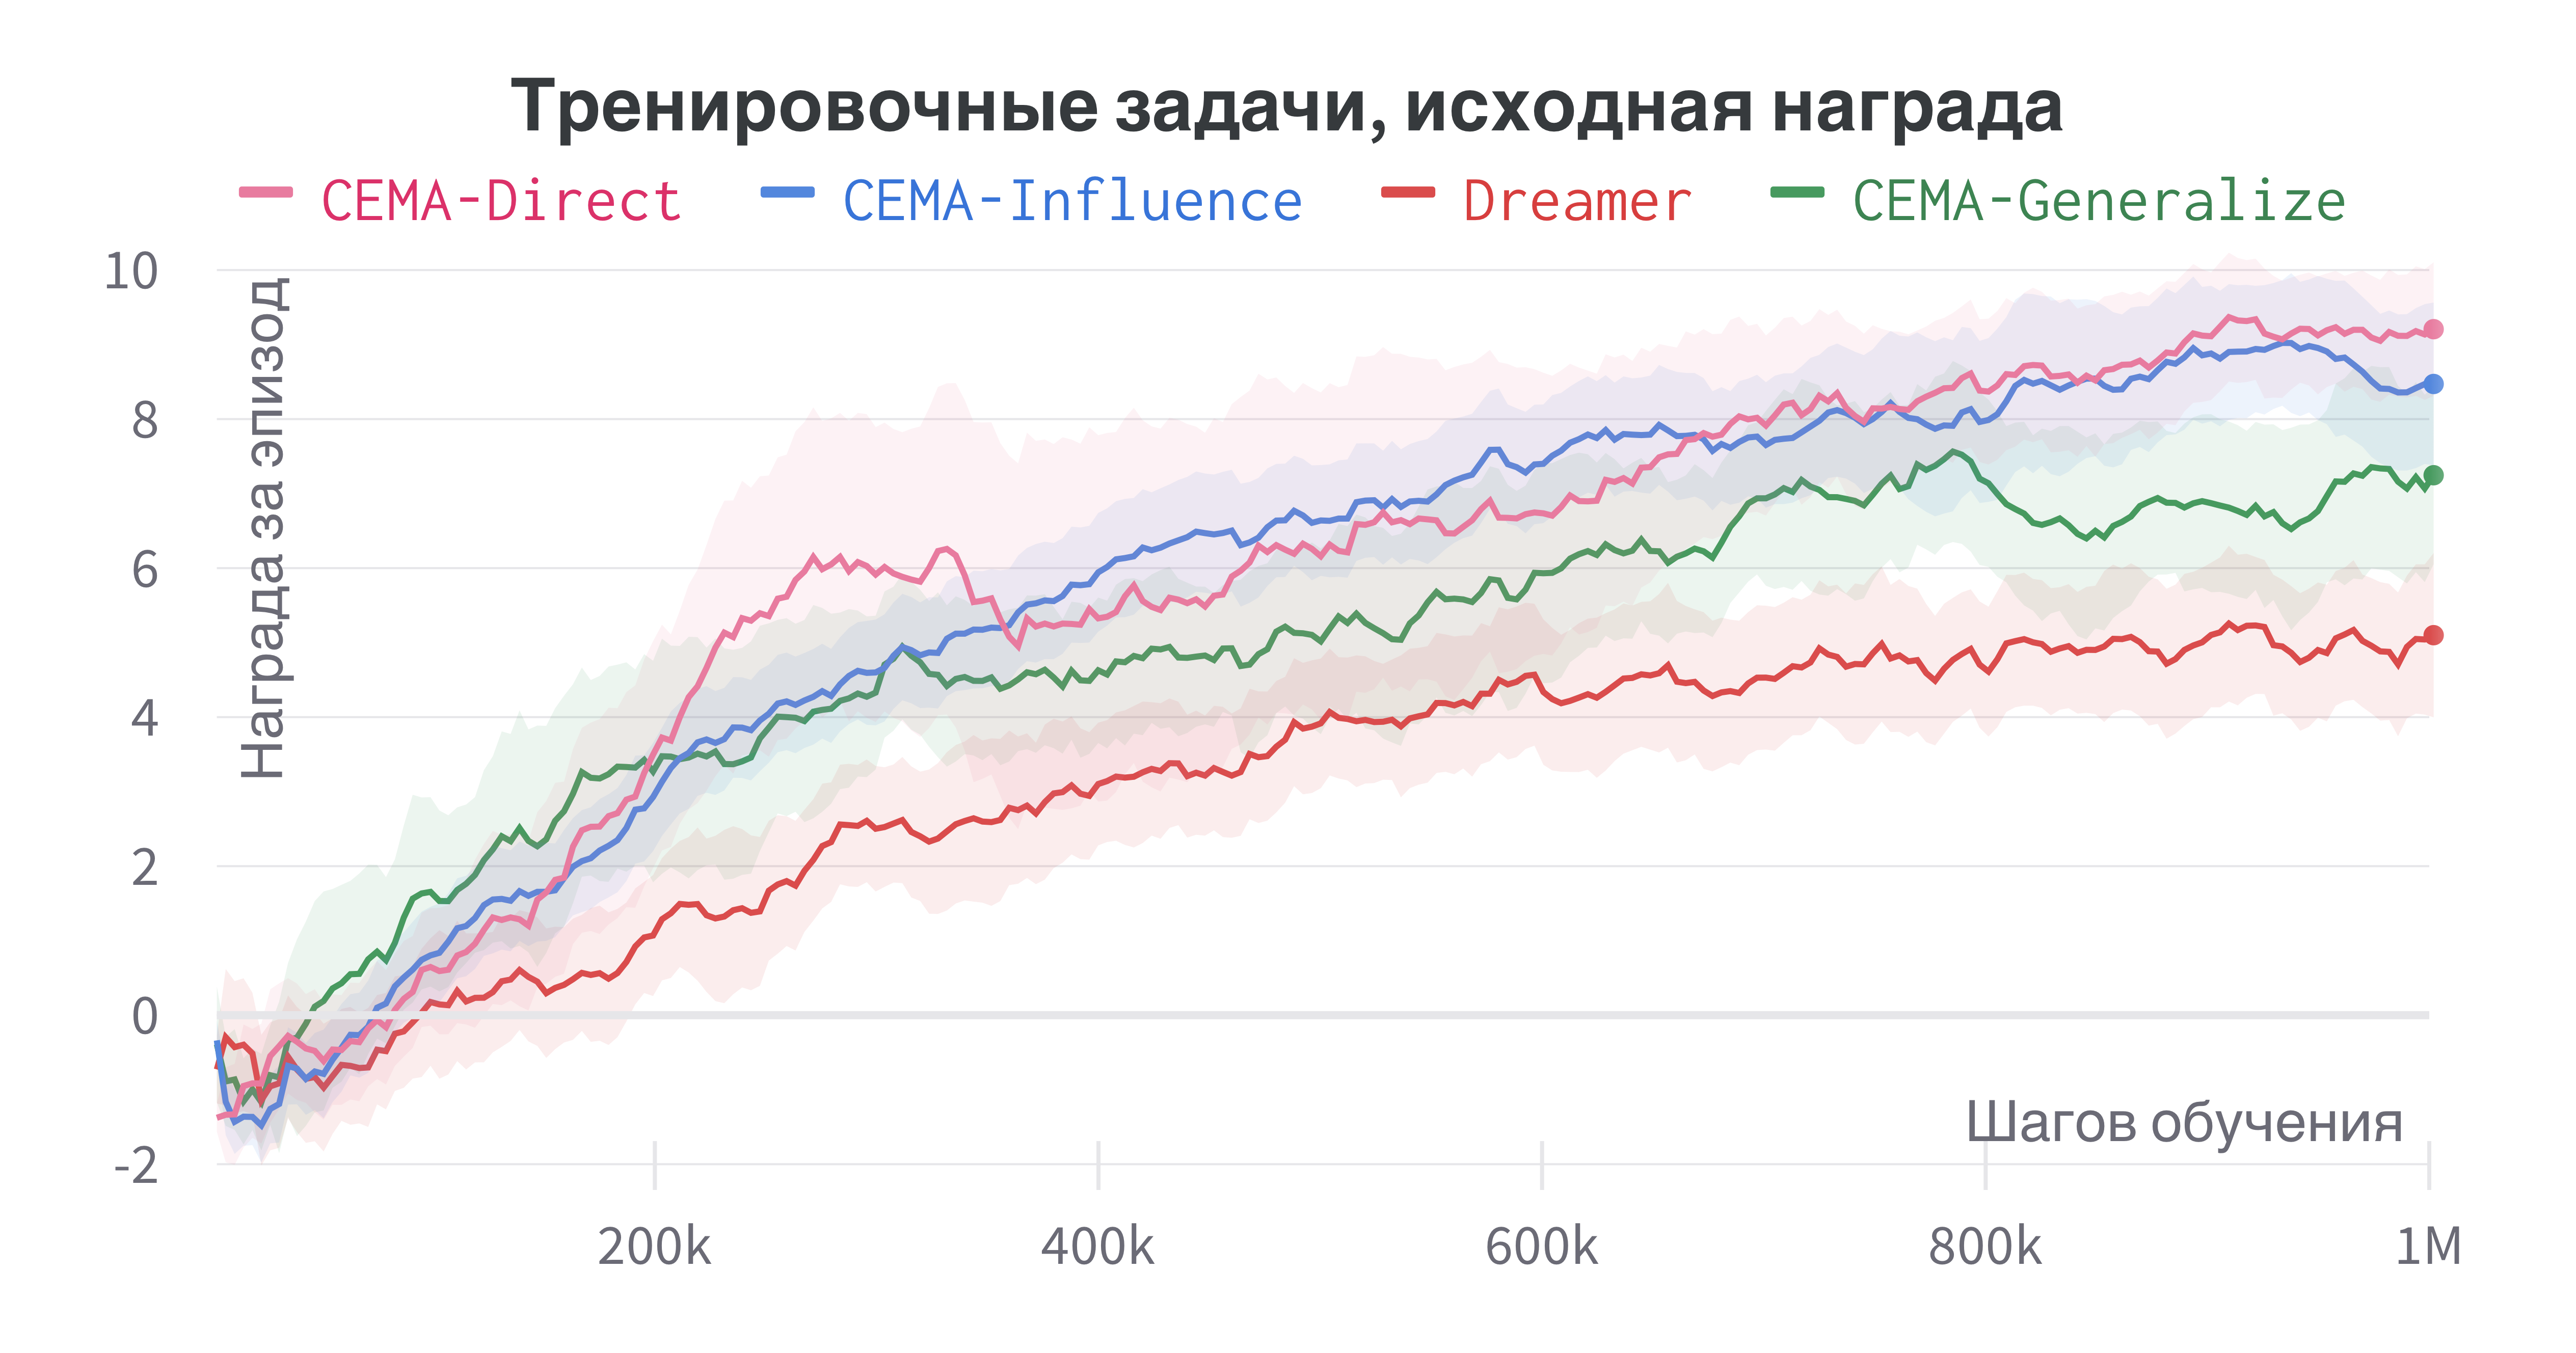
\includegraphics[width=\linewidth]{figures/cw_raw_train.png}
    \end{subfigure}
    \begin{subfigure}{.47\textwidth}
        \centering
        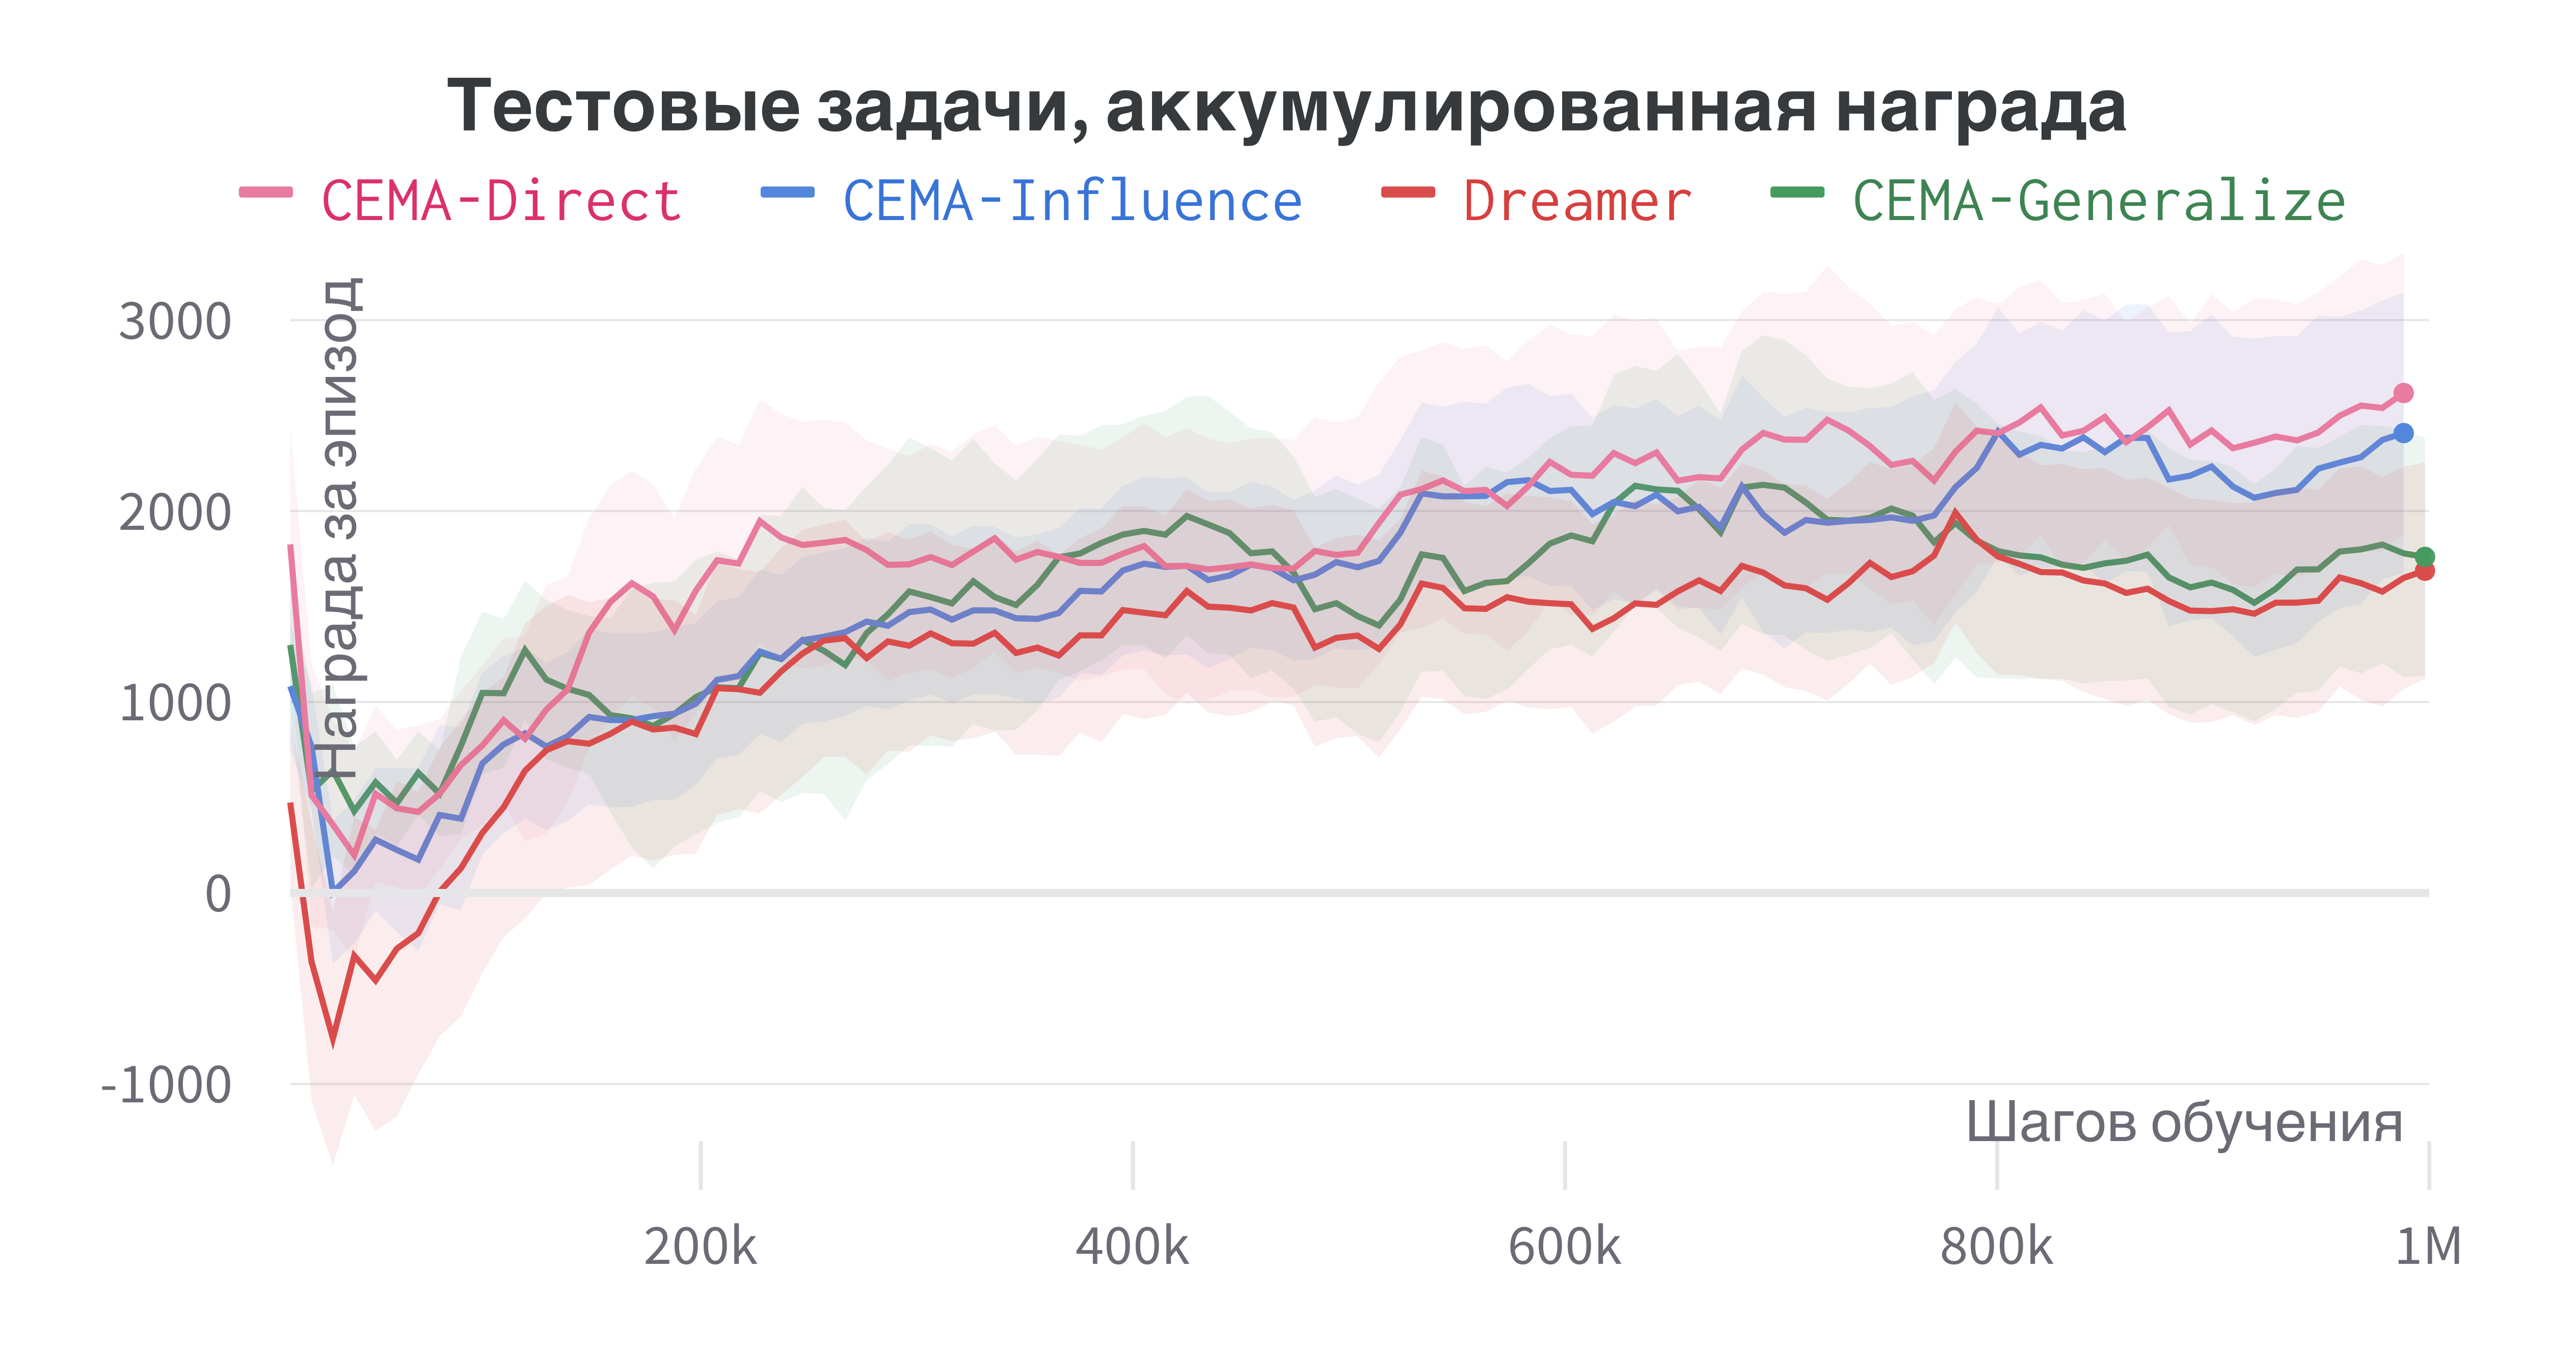
\includegraphics[width=\linewidth]{figures/cw_cum_test.png}
        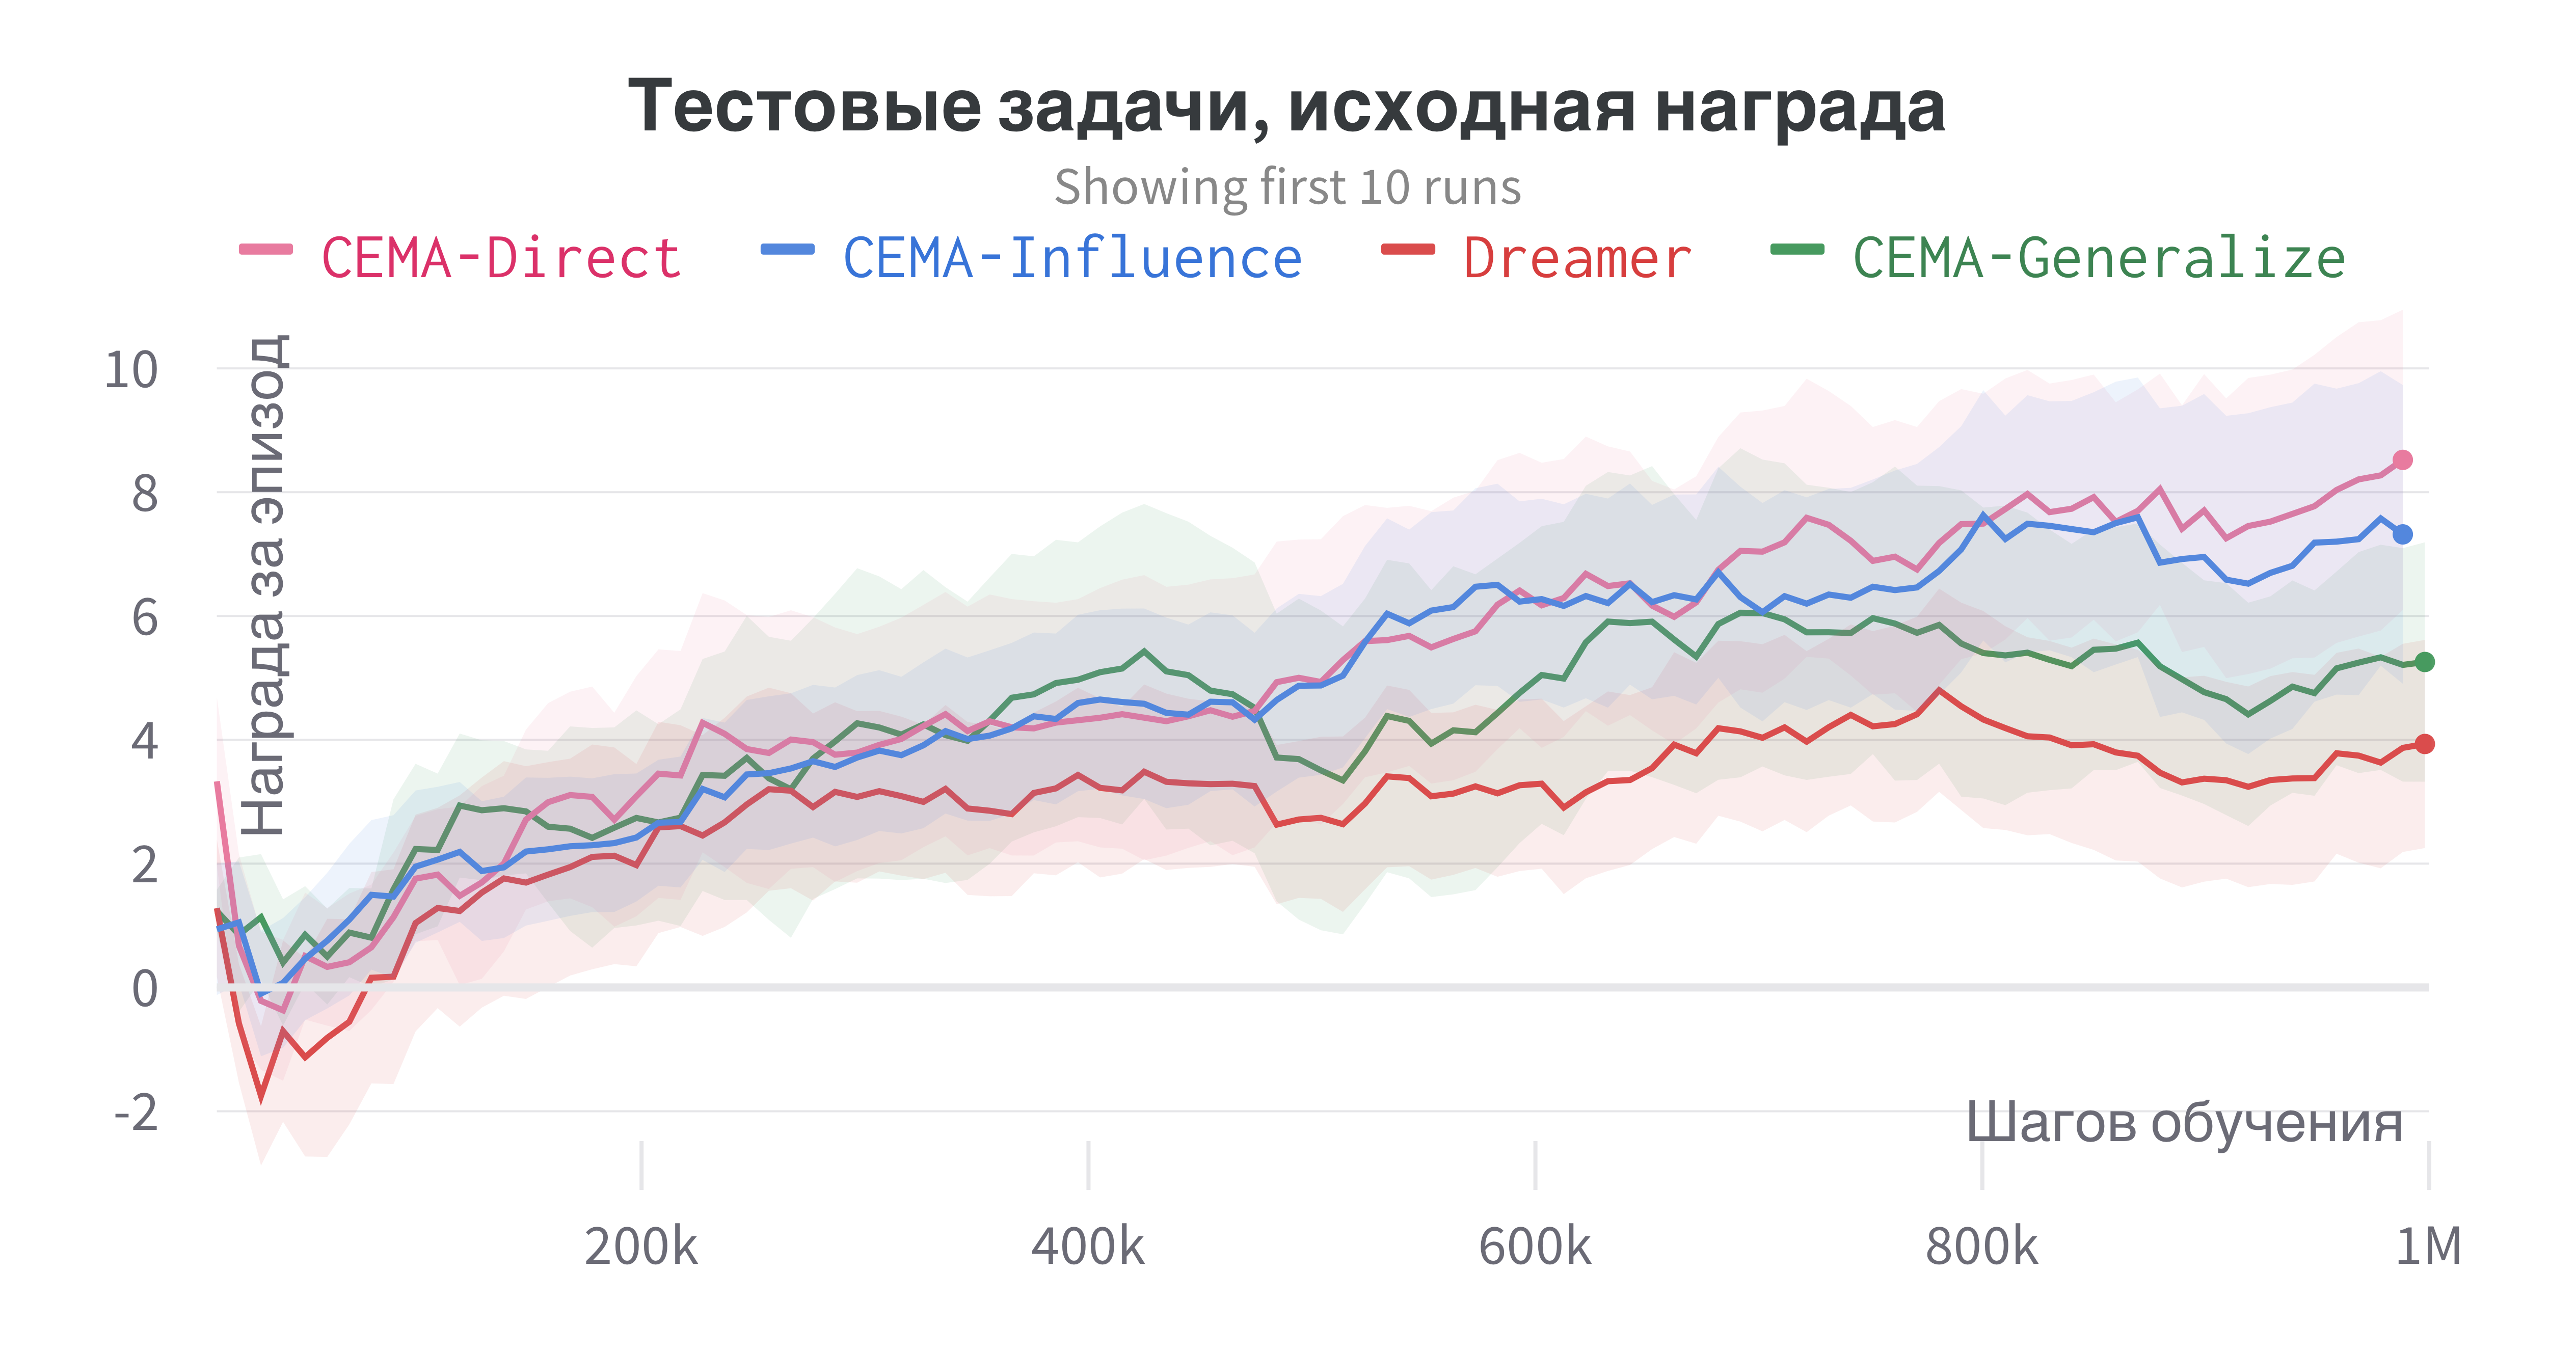
\includegraphics[width=\linewidth]{figures/cw_raw_test.png}
    \end{subfigure}
    \caption{Графики тренировочного процесса в среде Pushing библиотеки CasualWorld.}
    \label{fig:cw_res}
\end{figure}



\clearpage
%%%%%%%%%%%%%%%%%%%%%%%%%%%%%%%%%%%%%%%%%%%%%%%%%%%%%%%%%%%%%%%%%%%%%%%%%%
\section{Заключение}
%%%%%%%%%%%%%%%%%%%%%%%%%%%%%%%%%%%%%%%%%%%%%%%%%%%%%%%%%%%%%%%%%%%%%%%%%%

% В~заключении конспективно перечисляются результаты, выносимые на~защиту.

% Пример:

% \paragraph{Основные результаты работы}
% \begin{itemize}
% \item
%     Предложен новый подход к\dots Доказано, что\dots 
% \item
%     Разработаны и реализованы алгоритмы\dots
% \item
%     Проведены вычислительные эксперименты\dots,
%     которые подтвердили / опровергли гипотезу о~том, что\dots
% \end{itemize}

% В~заключении можно также перечислить предполагаемые направления дальнейших исследований.

В настоящей работе были предложены и описаны объектно-центричные модели мира в обучении с подкреплением для алгоритмов модельного подхода, решающих задачу визуального роботизированного контроля. За счет предположения о работе только с манипулятором и объектом, стало возможным внести в структуру в явном виде предположения о причинно-следственных связях в среде. Благодаря подобному моделированию, а также благодаря модификациям, свойственным только объектно-центричным моделям мира, было достигнуто улучшение обобщающей способности базового алгоритма.

Предложенное направление исследований представляется весьма перспективным, поскольку применение объектно-центричного подхода в других областях науки уже доказало его состоятельность. В настоящей работе была показана возможность добиться улучшений обобщающей способности алгоритмов, но при этом присутствовал ряд существенных ограничений, ограничивающих применение алгоритма для реальных задач.

Таким образом, для дальнейших исследований можно выделить следующие направления:
\begin{enumerate}
    \item избавиться от необходимости использовать истинные сегментационные маски в алгоритме;
    \item исследовать возможности интеллектуальной активации вектора влияния в моменты взаимодействия манипулятора с объектом;
    \item рассмотреть случай с большим количеством объектов и/или манипуляторов;
    \item рассмотреть возможные применения объектно-центричного подхода для улучшения иных качеств алгоритмов обучения с подкреплением.
\end{enumerate}

\clearpage

\bibliographystyle{gost71s}
\bibliography{biblio}

\end{document}
